\documentclass[12pt,fleqn,a4paper,nodisplayskipstretch]{article}
\usepackage[a4paper, left=30mm, right=20mm, top=30mm, bottom=20mm]{geometry}
\usepackage{geometry}
\usepackage{float}
\usepackage{url}
\usepackage{subfigure}
\usepackage{epsfig,float,amsmath,amsthm,graphicx,graphics,amssymb,amsfonts,newlfont,indentfirst}
\usepackage{fancyhdr}
\usepackage{ragged2e}
\usepackage{graphics}
\usepackage{diagbox}
\usepackage{tabularx}
\usepackage{minitoc}
\usepackage[utf8]{inputenc}
\usepackage{ragged2e}
\usepackage{mathptmx}
\usepackage{nomencl}
\usepackage[brazil]{babel}
\usepackage[alf,abnt-repeated-title-omit=yes,abnt-emphasize=bf,abnt-etal-list=0]{abntex2cite}

\citebrackets()
\makenomenclature

\renewcommand{\footnoterule}{
\kern -3pt
\hrule width 5cm
\kern 2pt
}

\AtBeginDocument{
    %Centralização do título sumário
    \renewcommand\contentsname{\centering \normalsize \uppercase{Sumário}}
    %Renomeação do título das siglas
    \renewcommand{\nomname}{\centering \normalsize \uppercase{Siglas}} 
    %Remoção do título referências
    \renewcommand{\refname}{} 
    %Renomeação do título da lista de figuras
    \renewcommand{\listfigurename}{\centering \normalsize \uppercase{Lista de figuras}}
    %Renomeação do título da lista de tabela
    \renewcommand{\listtablename}{\centering \normalsize \uppercase{Lista de tabelas}}
}

\headheight=16pt
\pagestyle{fancy}
\fancyhf{}
\fancyheadoffset{0cm}
\renewcommand{\headrulewidth}{0pt} 
\renewcommand{\footrulewidth}{0pt}
\fancyhead[R]{\thepage}
\fancypagestyle{plain}{
  \fancyhf{}
  \fancyhead[R]{\thepage}
}


\begin{document}

{\setstretch{1.5}
\thispagestyle{empty}
\begin{center}
	{\bf Universidade Estadual Paulista\\
		Faculdade de Ciências e Tecnologia \\
	Departamento de Matemática e Computação}
\end{center}

\vspace{3cm} \begin{center}
{\bf Relatório Final}\\
Bolsa de Iniciação Científica --- PICME
\end{center}

\vspace{4cm}

{\Large\bf \noindent \begin{center} Métodos computacionais para solução de equações diferenciais ordinárias
	\end{center} }

\vspace{6cm}
\begin{quote}
	{\bf Bolsista:} Gustavo Becelli do Nacimento

	{\bf E-mail:} gustavobecelli@gmail.com

	{\bf Telefone:} (18) 99824-1708

	{\bf Orientadora:} Profa. Dra. Analice Costacurta Brandi

	{\bf Período:} 01 de agosto de 2021 a 31 de julho de 2022
\end{quote}


\pagebreak

\thispagestyle{empty}
\listoffigures{}
\pagebreak

\thispagestyle{empty}
\listoftables{}
\pagebreak

\pagenumbering{arabic}
\tableofcontents{}
\pagebreak



% Apresentar uma panorâmica da área a ser estudada, descrevendo o histórico da área, o cenário atual, os problemas existentes, o objetivo deste trabalho e, no final, a estrutura deste documento, descrevendo brevemente os demais capítulos desta revisão.

\section{Introdução} \label{introduction}
O Inpainting  de Imagens é o processo de preencher regiões faltantes ou danificadas de uma imagem com o intuito de restaurá-la ou melhorar sua aparência. Este é um problema amplamente estudado em visão computacional e possui uma vasta gama de oportunidades de aplicações, incluindo o restauro de obras artísticas e fotografias danificadas, a remoção de objetos de imagens e síntese de texturas~\cite{criminisi2004region}.

Esta área de pesquisa tem sido estudada há várias décadas. Os primeiros trabalhos sobre o tema surgiram na década de 1950, mas foi somente a partir dos anos 1990 que o inpainting começou a ser utilizado de maneira mais ampla.

\cite{Elharrouss2019} apresenta uma revisão sobre o inpainting de imagens, descrevendo os principais métodos e aplicações. Neste campo, existem várias técnicas para o inpainting de imagens, cada tal com suas próprias vantagens e desvantagens. Uma abordagem popular é apresentada em \cite{Bertalmio2000}, a qual introduz uma técnica de inpainting baseada no conceito de complementar uma região de uma imagem existente. Neste trabalho é utilizado equações diferenciais parciais para propagar informações das bordas da região danificada para o centro da região, permitindo que o algoritmo estime como os pixels devem ser restaurados.

Uma das contribuições mais significativas para o campo de inpainting de imagem é o desenvolvimento do ``Método de Marcha Rápida'' ~\cite{Telea2004}, um algoritmo eficiente que usa equações diferenciais parciais para propagar informações de pixels conhecidos para os pixels desconhecidos na região de inpainting. Este algoritmo tem sido amplamente utilizado em várias aplicações e foi implementado em muitas bibliotecas de software, incluindo a biblioteca de código aberto de visão computacional OpenCV \cite{OpenCV}. Este método tem demonstrado produzir resultados de alta qualidade para uma ampla variedade de tipos de imagem e cenários, e se tornou uma das referências para avaliar o desempenho de outros algoritmos de inpainting.

Nos últimos anos, houve um aumento de interesse em utilizar métodos baseados em aprendizado de máquina, como redes adversárias gerativas (GANs) e redes neurais convolucionais (CNNs) \cite{pathakCVPR16context}, para resolver o problema de inpainting. Esses métodos têm o potencial de aprender padrões e estruturas complexas a partir de grandes conjuntos de dados, o que pode ser usado para gerar resultados de inpainting de alta qualidade. No entanto, esses métodos podem ser computacionalmente caros e podem exigir uma abundância de dados de treinamento para obter bons resultados.

Hoje, o inpainting é utilizado em uma variedade de aplicações. Dentre elas, está incluída o restauro de obras de arte danificadas, a remoção de objetos de imagens (como nuvens em imagens de sensoriamento remoto) e até mesmo a
remoção de imperfeições de fotografias. Além disso, pode-se utilizar os mesmos conceitos de restauração para modificar as perspectivas de imagens, como é apresentado em \cite{huang2014image}.

O principal problema encontrado neste campo de pesquisa são a escolha do método de inpainting mais adequado para cada tipo de imagem e cenário. Este fator se deve às desvantagens que os métodos existentes proporcionam \cite{Salem2021}. Em geral, os maiores desafios são:
\begin{itemize} 
  \item \textbf{Preservação da consistência e estrutura da imagem de entrada:} muitos modelos geradores podem gerar imagens visualmente agradáveis, mas que não correspondem perfeitamente com a vizinhança ou à textura da imagem original.
  \item \textbf{Preservação de pequenos detalhes:} este problema é particularmente desafiador para imagens com texturas complexas, como imagens de paisagens naturais, ou a área que está sendo restaurada é muito grande.
  \item \textbf{Reconstruir objetos sobrepostos:} quando um objeto é parcial ou completamente sobreposto, como um objeto que está coberto por uma nuvem, o modelo gerador pode não ser capaz de reconstruir o objeto original.
  \item \textbf{Preenchimento de grandes regiões:} a geração de imagens de alta qualidade quando há uma grande região a ser reconstruída ainda é um problema desafiador.
  \item \textbf{Desempenho computacional:} a maioria dos métodos de inpainting de imagens que geram imagens de alta qualidade são computacionalmente caros, dificultando sua aplicação em tempo real.
\end{itemize}


\subsection{Objetivos}

\subsubsection{Objetivo principal}
O objetivo principal deste Trabalho de Conclusão de Curso é investigar e implementar algumas das diferentes técnicas de Inpainting para a restauração de imagens digitais com defeitos ou objetos indesejados. Para alcançar esse objetivo, serão estudadas técnicas clássicas baseadas em informações de vizinhança e amostras, bem como técnicas mais recentes baseadas em aprendizado de máquina. Além disso, serão aplicadas as técnicas estudadas em diversos tipos de imagens para avaliar sua eficácia e comparar os resultados obtidos.

\subsubsection{Objetivos secundários}
\begin{itemize}
  \item Estudar alguns dos principais métodos de inpainting, com o intuito de entender como cada um deles funciona e quais são suas vantagens e desvantagens.
  \item Aplicar as técnicas de inpainting estudadas em diversos tipos de imagens, incluindo imagens coloridas, imagens de alta resolução e imagens com diferentes tipos de defeitos, como buracos, riscos, manchas, etc.
  \item Aperfeiçoar os conhecimentos em processamento de imagens e aprendizado de máquina do aluno, bem como a capacidade de aplicar esses conhecimentos em problemas reais.
  \item Estudar a possibilidade de melhorias na eficácia (qualidade das imagens geradas) e na eficiência (tempo de processamento, uso de memória) dos métodos de inpainting estudados.
\end{itemize}

Os três objetivos secundários representam o âmbito deste trabalho dentro do objetivo principal. O último, por sua vez, representa o interesse do aluno em aprofundar seus conhecimentos em otimização computacional de algoritmos e a possibilidade de contribuir com a comunidade científica.

\subsection{Organização do Trabalho}
Inicialmente apresenta-se uma fundamentação teórica sobre o processo de inpainting, incluindo uma breve introdução sobre o escopo de inpainting, as principais categorias da área e posteriormente uma revisão de alguns dos principais métodos utilizados.
Em seguida, há uma seção destinada a mencionar algumas possíveis técnicas de otimização computacionais que podem ser aplicadas caso haja a possibilidade de serem implementadas.

Por fim, é apresentado um 
\section{Plano de Trabalho e Cronograma}\label{sec:cronograma}

Este trabalho tem como objetivo desenvolver e implementar algoritmos numéricos para a solução de equações diferenciais ordinárias (EDOs) utilizando a linguagem de programação \emph{Python} e as bibliotecas numéricas \emph{NumPy} e \emph{Numba}. Para alcançar esse objetivo, foi realizada uma revisão bibliográfica a fim de adquirir uma fundação teórica no domínio do problema, com foco no estudo de equações diferenciais e métodos iterativos explícitos e implícitos.

Para verificar a precisão e confiabilidade do código, os testes do algoritmo começarão com problemas mais simples, com soluções analíticas ou numéricas conhecidas. Em seguida, serão realizados testes preliminares para verificar o código, usando diferentes condições iniciais e comparando os resultados com a literatura existente. Finalmente, será realizada uma análise dos erros obtidos, da convergência e do tempo computacional.

Durante todo o processo, será redigido um relatório das atividades para documentar e apresentar os resultados obtidos. O uso do compilador JIT \emph{Numba} também será considerado para melhorar o desempenho computacional do algoritmo.

Este projeto de pesquisa foi desenvolvido em um período de doze meses e dividido em oito etapas:

\begin{enumerate}
	\item Revisão bibliográfica: realização de pesquisa bibliográfica em livros e artigos científicos para adquirir fundamentação teórica no domínio do problema.
	\item Implementação das equações diferenciais em linguagem computacional: codificação dos modelos matemáticos das equações diferenciais ordinárias, utilizando as bibliotecas \emph{Numpy}, \emph{Numba} e a linguagem de programação \emph{Python}.
	\item Estudo e implementação dos métodos numéricos iterativos e de diferenças finitas: estudo e implementação de métodos numéricos iterativos e de diferenças finitas para solucionar as equações diferenciais implementadas.
	\item Estudo e uso de um método de solução de sistema de equações não lineares: estudo e implementação de um método de solução de sistema de equações não lineares para tratar equações diferenciais implícitas.
	\item Testes preliminares para constatação da acurácia do código: realização de testes com problemas mais simples para verificar a precisão do código implementado.
	\item Testes numéricos para validação dos métodos iterativos: execução de testes numéricos para validar os métodos implementados, utilizando diferentes condições iniciais e sendo comparados com resultados da literatura.
	\item Análise dos resultados obtidos: análise dos erros obtidos, da convergência e do tempo computacional dos métodos numéricos iterativos e de diferenças finitas implementados.
	\item Relatório Final: redação do relatório final das atividades realizadas, contendo a descrição detalhada dos métodos implementados e resultados obtidos.
	\end{enumerate}
\subsection{Formulação Matemática}\label{sec:mathematical_formulation}
Esta seção apresenta a formulação matemática dos problemas em estudo. Para tanto, são utilizadas equações diferenciais ordinárias que descrevem o crescimento de uma ou mais populações. É importante ressaltar que essas equações podem envolver variáveis dependentes de ordem superior e que, geralmente, é conhecida a população inicial, também chamada de condição inicial.

Formalmente, temos que os problemas estudados podem ser descritos por equações da forma:

\begin{equation*}
\dfrac{dy}{dx} = f(x,y)
\end{equation*}

onde $y$ representa a(s) população(ões) em estudo e $x$ representa o tempo. A função $f(x,y)$ determina a taxa de crescimento ou decrescimento da população em relação ao tempo.
\section{Formulação Numérica}\label{sec:formnumer}

Nesta seção, são descritos os métodos numéricos utilizados para resolver equações diferenciais. Quando a solução analítica não é conhecida ou é muito complexa de ser resolvida, os métodos iterativos são uma alternativa para se obter uma solução aproximada. Para isso, a discretização do domínio é realizada, dividindo-o em uma malha fixa ou variável, dependendo do método utilizado.

Vale ressaltar que, embora os métodos explícitos, como o de Euler Explícito, sejam computacionalmente mais eficientes, eles geralmente sofrem de maior instabilidade em problemas rígidos (\emph{stiff}), enquanto os métodos implícitos, como o de Euler Implícito, são mais estáveis em tais casos \cite{ascher2008numerical}. No entanto, este trabalho não abordará problemas rígidos.


\subsection{Método de Diferenças Finitas e Polinômio de Taylor} \label{sec:finite_differences}

O método de diferenças finitas consiste em discretizar o domínio do problema, gerando uma malha de pontos que será utilizada para aproximar a função original por meio da expansão do polinômio de Taylor. O polinômio de Taylor é uma série infinita que representa a função em torno de um ponto $x_0$, podendo ser truncado para viabilizar o cálculo computacionalmente.

A expansão do polinômio de Taylor de ordem $n$ em relação a uma variável $h$ é dada por:

\begin{equation*} \label{taylor}
f(x+h)= f(x) + hf'(x) + \frac{h^2}{2!}f''(x)+...+ \frac{h^n}{n!}f^{(n)}(x) + \frac{h^{n+1}}{(n+1)!}f^{(n+1)}(x)
\end{equation*}

O erro global do polinômio de grau $n$ na variável $h$ é dado por $\frac{h^{n+1}}{(n+1)!}f^{(n+1)}(x)$. A ordem do erro é classificada conforme o expoente de $h$. É importante notar que, quanto menor for o valor de $h$, menor será o erro, e os métodos de maior ordem geralmente possuem maior precisão em comparação aos métodos de ordem inferior.

O refinamento da malha é fundamental para o sucesso das aproximações, pois quanto menor for o incremento $h$, mais próximo será o valor estimado da diferenciação exata. Entretanto, é importante destacar que o processo de truncamento introduz pequenos erros no cálculo da aproximação, o que pode acumular e levar à não-convergência do método. Portanto, é crucial avaliar a ordem do método utilizado de acordo com o problema a ser resolvido e a tolerância de erro aceita.


\subsubsection{Diferenças Avançadas}\label{sec:difavan}

As diferenças avançadas recebem este nome pois aproximam a derivada do ponto $x_i$ por meio da diferenciação conforme um incremento de $h$, ou seja, calculando em um ponto adiante de $x_i$. Considerando a função $f(x)$, é possível aproximar sua derivada por meio de um desenvolvimento no polinômio de Taylor \cite{leveque2007finitediff}. Para $n=1$ e $x=x_i$ um ponto da malha, tem-se:

\begin{equation*}
f(x_i+h)= f(x_i)+ hf'(x_i) + \frac{h^2}{2!}f''(\xi)
\end{equation*}

com $\xi$ entre $x_i$ e $x_i + h$. Isolando $f'(x_i)$, obtemos:

\begin{equation*}
f'(x_i)= \frac{f(x_i+h)-f(x_i)}{h} + \frac{h}{2}f''(\xi)
\end{equation*}

ou

\begin{equation*}
f'(x_i)= \frac{f(x_i+h)-f(x_i)}{h} + O(h)
\end{equation*}

Observa-se que este processo define o método de diferenças avançadas, que aproxima a derivada computando o diferencial de $x_i$ e $x_i + h$. O erro global das diferenças avançadas é de primeira ordem, conforme o expoente $1$ que acompanha $h$.

Para representação computacional, o método de diferenças avançadas em notação de índices é dado, após ignorar o termo de erro, por:

\begin{equation}\label{forward_diff}
f'(x_i)= \frac{f(x_{i+1})-f(x_i)}{h}
\end{equation}

É importante notar que o incremento $h$ escolhido para a aproximação deve ser cuidadosamente selecionado, levando em conta o compromisso entre a precisão da solução e a resolução da malha.

\subsubsection{Diferenças Atrasadas}\label{sec:bw_diff}

As diferenças atrasadas são um método para aproximar a derivada em um ponto $x_i$ usando um decremento $h$ na variável $x$, isto é, calculando o diferencial em um ponto anterior a $x_i$. Este método é obtido através do desenvolvimento da série de Taylor da função $f(x)$ no ponto $x_i$:

\begin{equation*}
f(x_i-h)= f(x_i)- hf'(x_i) + \frac{h^2}{2!}f''(\xi),
\end{equation*}

onde $\xi$ está entre $x_i-h$ e $x_i$. Isolando $f'(x_i)$, temos:

\begin{equation*}
f'(x_i)= \frac{f(x_i)-f(x_i-h)}{h} + \frac{h}{2}f''(\xi)
\end{equation*}

ou, de forma mais concisa,

\begin{equation*}
f'(x_i)= \frac{f(x_i)-f(x_i-h)}{h} + O(h)
\end{equation*}

Observamos que este é o método de diferenças atrasadas, que aproxima a derivada usando uma diferença finita regressiva. Este método possui erro de primeira ordem, que é proporcional a $h$.

Em notação de índices, o método de diferenças atrasadas é, após ignorar o termo de erro, dado por:

\begin{equation}\label{backward_diff}
f'(x_i)= \frac{f(x_{i})-f(x_{i-1})}{h}
\end{equation}

\subsubsection{Diferenças Centradas}\label{sec:ct_diff}

As diferenças centradas recebem esse nome porque são a média ou o centro dos métodos de diferenças avançadas e atrasadas. Essas diferenças são calculadas fazendo a média dos pontos anteriores e posteriores a $x$. Para $n = 2$ em (\ref{taylor}) e tomando $h$ e $-h$, temos:

\begin{equation}\label{central_diff_forward}
f(x_i+h) = f(x_i) + hf'(x_i) + \frac{h^2}{2!}f''(x_i) + \frac{h^3}{3!}f'''(\xi_1)
\end{equation}
onde $\xi_1$ está entre $x$ e $x+h$.
\begin{equation}\label{central_diff_backward}
f(x_i-h) = f(x_i) - hf'(x_i) + \frac{h^2}{2!}f''(x_i) - \frac{h^3}{3!}f'''(\xi_2)
\end{equation}
onde $\xi_2$ está entre $x-h$ e $x$.

Subtraindo (\ref{central_diff_backward}) de (\ref{central_diff_forward}), temos:

\begin{equation}\label{central_diff_opened}
f(x_i+h) - f(x_i-h) = 2hf'(x_i) + \frac{h^3}{3!}\big(f'''(\xi_1) + f'''(\xi_2)\big)
\end{equation}
De acordo com o Teorema do Valor Intermediário, $\frac{f'''(\xi_1)+ f'''(\xi_2)}{2}= f'''(\xi)$, onde $\xi$ está entre $x-h$ e $x+h$.

Isolando a primeira derivada em (\ref{central_diff_opened}), temos:

\begin{equation*}
f'(x_i)= \frac{f(x_i+h)-f(x_i-h)}{2h} - \frac{h^2}{3!}f'''(\xi)
\end{equation*}
Observa-se que este método pertence à família de métodos de ordem 2, dependendo do expoente de $h$. Isso pode ser denotado como:

\begin{equation*}
f'(x_i)= \frac{f(x_i+h)-f(x_i-h)}{2h} +O(h^2)
\end{equation*}

Ou apenas em notação de índices:

\begin{equation}\label{central_difference}
f'(x_i)= \frac{f(x_{i+1})-f(x_{i-1})}{2h}
\end{equation}

Os métodos de diferenças centradas também apresentam uma aproximação para a segunda derivada de $f(x)$, também de ordem 2. Para obter essa aproximação, equacionamos (\ref{central_diff_backward}) e (\ref{central_diff_forward}) para eliminar a primeira derivada e isolar a segunda. Dessa forma, obtemos a seguinte aproximação para $f''(x)$:

\begin{equation*}\label{cd_2nd_derivative}
	f''(x) = \frac{f_{i+1}  - 2f_{i} + f_{i-1}}{h^2} + O(h^2)
\end{equation*}


\subsection{Problema de Valor Inicial}\label{sec:ivp}
Os Problemas de Valor Inicial (PVI) consistem em uma equação diferencial e uma condição inicial, em um dos limites do intervalo. O objetivo é encontrar o valor da função-problema $y(x)$ ao longo do intervalo $[a, b]$ do problema, com $a, b \in \mathbb{R}$, a partir da condição inicial. Para isso, usa-se um método numérico que aproxima os valores da função-problema em pontos discretos do intervalo, a partir da diferença aproximada pela derivada. Um PVI é representado por:
\begin{equation*}
	\begin{cases}
		y' = f(x,y) &                           \\
		y(a) = y_a  & \text{ com } x \in [a, b] 
	\end{cases}
\end{equation*}

Assumindo que $y(x_0) = y_0$, é possível aproximar $y(x)$ com uma expressão do tipo:
\begin{equation*}
y_{i+1} = y_i + Z \text{ com } i = 0, 1, ..., N \text{ e } Z, N \in \mathbb{R}
\end{equation*}
Neste exemplo, $Z$ é a diferença calculada pelo método entre os pontos $y_i$ e $y_{i+1}$.

Para garantir a existência e unicidade da solução, assume-se que o PVI satisfaz a condição de Cauchy-Lipschitz. Com isso, pode-se afirmar que:
\begin{enumerate}
\item $y(x)$ é contínua e diferenciável no intervalo $[a, b]$;
\item $y(a) = y_a$;
\item $y'(x) = f(x, y(x))$, com $x \in [a, b]$.
\end{enumerate}

\subsection{Métodos de Euler e Runge-Kutta}\label{sec:ivp_methods}
Nesta subseção, serão apresentados os métodos para integrações numéricas de equações diferenciais ordinárias. Conforme discutido em (\ref{sec:finite_differences}), há três métodos de diferenças finitas para aproximar as derivadas, mas somente com eles não é possível realizar o processo inverso de integração numérica através da derivada. No entanto, caso a equação diferencial ordinária seja um PVI, é possível aproximar sua antiderivada numericamente por meio de manipulações nos métodos de diferenças finitas.

Além disso, serão abordados os métodos de Runge-Kutta de ordem $n>1$, que utilizam o declive da função em pontos específicos do intervalo [$x_i$,$x_{i+1}$] para aprimorar a aproximação. Ao contrário do método de Euler explícito de primeira ordem, os métodos de Runge-Kutta de ordem superior usam uma combinação ponderada de declives em vários pontos para obter uma melhor aproximação numérica. 


\subsubsection{Método de Euler explícito}\label{sec:explicit_euler}

O método de Euler explícito, também conhecido como método de Runge-Kutta explícito de primeira ordem, é uma técnica utilizada para resolver equações diferenciais ordinárias. Ele é obtido a partir da equação (\ref{forward_diff}), sendo dado por:
\begin{equation}\label{explicit_euler}
y_{i+1}= y_{i} + h f(x_i, y_i)
\end{equation}
onde $i = 0, 1,...,N$, sendo $i$ a iteração e $N \in \mathbb{N}^*$. Observa-se que o ponto da iteração $y_{i+1}$ é calculado explicitamente a partir do valor de $y_i$, para qualquer que seja $f(x_i, y_i)$. Devido à propriedade de calcular o próximo passo com o atual, este método é classificado como explícito.

O método de Euler explícito aproxima um ponto da função original somando o valor do ponto anterior ao produto do espaçamento da malha $h$ e da derivada da função no ponto anterior. O erro global deste método é de primeira ordem.

\subsubsection{Método de Euler implícito}\label{sec:implicit_euler} \quad

Analogamente a (\ref{explicit_euler}), este método pode ser obtido equacionando (\ref{backward_diff}) e incrementando em 1 o índice $i$:
\begin{equation}\label{implicit_euler}
	y_{i}= y_{i-1} + hy'_{i} \implies y_{i+1}= y_{i} + hy'_{i+1}
\end{equation}
com $i = 0, 1,...,N$ sendo $i$ a iteração e $N \in \mathbb{N}^*$. Observa-se que por tratar-se de uma equação diferencial, $y'_i$ é definida como $y'(x_i, y_i)$. Por consequência, a variável dependente $y_{i+1}$ está presente em ambos lados da equação. Para solucionar este problema, é necessário resolver um sistema de equações não-lineares.
Exemplificando o processo, caso o PVI dado seja:
\begin{equation*}
	\begin{cases}
		y' = x + y &                           \\
		y(0) = 0   & \text{ com } x \in [0, 1] 
	\end{cases}
\end{equation*}
Ao substituir a derivada no método de Euler implícito, obtemos a seguinte fórmula implícita:
\begin{equation*}
	y_{i+1} = y_i + h f(x_{i+1}, y_{i+1}) \\
	\iff y_{i+1} = y_i + h (x_{i+1} + y_{i+1})\\ 
\end{equation*}
Reorganizando a equação, pode-se escrevê-la como:
\begin{eqnarray*}
	y_{i+1} = y_i + h (x_{i+1} + y_{i+1})\\
	\iff y_{i+1} = y_i + hx_{i+1} + hy_{i+1}\\
	\iff y_{i+1} - hy_{i+1} = y_i + hx_{i+1}\\
	\iff (1-h)y_{i+1} = y_i + hx_{i+1}\\
	\iff y_{i+1} = \frac{y_i + hx_{i+1}}{1-h}\qedhere
\end{eqnarray*}

Essa fórmula nos permite obter o valor de $y_{i+1}$ a partir de $y_i$ e $x_{i+1}$.

Em termos de implementação computacional, a equação não-linear do método de Euler implícito pode ser resolvida por meio do método de iteração de ponto fixo, que adiciona um custo computacional ao método. Porém, esse método é conhecido por ser mais estável que o método de Euler explícito, especialmente para EDOs que possuem soluções oscilatórias ou instáveis.


\subsubsection{Método do ponto médio modificado}\label{sec:modified-midpoint} \quad

O método do ponto médio modificado é uma variação dos métodos de Euler Explícito e Implícito. Ele é derivado do método de diferenças centradas (\ref{central_difference}) e possui um erro global de ordem 2. Sua forma geral pode ser escrita como:
\begin{equation*}
y_{i+1} = y_{i-1} + 2 h f'i
\end{equation*}
onde $i = 1, 2,...,N$ é o índice da iteração e $N \in \mathbb{N}^*$ é o número de iterações. É importante notar que, como o método depende de $y{i-1}$ e $f'_i$, é necessário que se tenha conhecimento prévio de $y_0$ e $y_1$ para iniciar a iteração. Como os problemas de valor inicial fornecem apenas o valor de $y_0$, o valor de $y_1$ é aproximado utilizando-se o método de Euler Implícito.

\subsubsection{Método de Runge-Kutta de terceira ordem}\label{sec:3rd-order-runge-kutta} \quad

O método de Runge-Kutta de terceira ordem é uma técnica computacional que utiliza variáveis auxiliares e temporárias para armazenar temporariamente um resultado previamente calculado. Essas variáveis são usadas para calcular um ponto intermediário entre o atual e o próximo, reduzindo assim a quantidade de processamentos redundantes e acelerando a execução.

Para obter a aproximação para o ponto $y_{i+1}$, é realizada uma média ponderada de três incrementos em $y_i$, sendo cada um deles um produto da estimativa do declive (ou coeficiente angular) em um ponto intermediário entre $y_i$ e $y_{i+1}$. Especificamente, $k_1$ é o coeficiente angular no início do intervalo, $k_2$ é um coeficiente no ponto médio do intervalo calculado usando $k_1$, e $k_3$ é o declive em três quartos do intervalo, que usa $k_2$ para ser calculado. Para avaliar a média ponderada, é dado maior peso para os declives a partir do ponto médio do intervalo.

Assim, a aproximação para $y_{i+1}$ é dada por:

% TODO: FIX THIS 2023
% \begin{flalign}
% 	k_1 = f(x_i, y_i)\\
% 	k_2 = f\PC{x_i + \frac{1}{2}h,\space y_i + \frac{k_1}{2}h}\\
% 	k_3 = f\PC{x_i + \frac{3}{4}h,\space y_i + \frac{3k_2}{4} h} \qedhere
% \end{flalign}
\begin{equation}
	y_{i + 1} = y_i + h \cdot \frac{(2k_1 + 3k_2 + 4k_3)}{9} \qedhere
\end{equation}

onde $i = 0, 1,...,N$, sendo $i$ a iteração e $N \in \mathbb{N}^*$. Observa-se que em uma única iteração, ambos os valores de $k_1$ e $k_2$ são utilizados duas vezes para aproximar $y_{i+1}$. Desta forma, o computador pode calcular o resultado uma única vez e utilizá-lo em ambas as ocorrências.
Este método de Runge-Kutta é de terceira ordem, isto é, seu erro global é $O(h^3)$ e oferece uma melhor aproximação da função original em comparação aos métodos de primeira e segunda ordem \cite{leveque2007finitediff}. Além disso, ele usufrui das vantagens dos cálculos computacionais para acelerar a execução.

\subsubsection{Método de Runge-Kutta de quarta ordem}\label{sec:4th-order-runge-kutta} \quad
O método de quarta ordem de Runge-Kutta é uma extensão/melhoria do método de terceira ordem e utiliza pontos pré-calculados para economizar processamento. Ele aproxima o valor de $y_{i+1}$ por meio de uma média ponderada de quatro incrementos em $y_i$, onde cada incremento é um produto da estimativa do declive (ou coeficiente angular) em um ponto intermediário entre $y_i$ e $y_{i+1}$.

$k_1$ é o coeficiente angular no início do intervalo. $k_2$ e $k_3$ são os coeficientes no ponto médio do intervalo, calculados usando $k_1$ e $k_2$, respectivamente. Já o coeficiente $k_4$ é o declive no final do intervalo e é calculado utilizando $k_3$. A média ponderada é calculada dando maior peso aos declives no ponto médio do intervalo. O método de quarta ordem é dado por:

\begin{equation}
\begin{aligned}
k_1 &= f(x_i, y_i)\
k_2 &= f\left(x_i + \frac{h}{2}, y_i + \frac{k_1}{2}h\right)\
k_3 &= f\left(x_i + \frac{h}{2}, y_i + \frac{k_2}{2}h\right)\
k_4 &= f\left(x_i + h, y_i + k_3h\right)
\end{aligned}
\end{equation}

\begin{equation}
	y_{i + 1} = y_i + \frac{h}{6}(k_1 + 2k_2 + 2k_3 + k_4)
\end{equation}

onde $i$ é a iteração e $N \in \mathbb{N}^*$ com $i = 0, 1,...,N$. Similarmente ao método de terceira ordem, os coeficientes $k_1$, $k_2$ e $k_3$ são reaproveitados para os próximos cálculos. O método de quarta ordem é mais preciso que o método de terceira ordem, com um erro global de $O(h^4)$, o que o torna adequado para resolver problemas que exigem maior precisão.

\subsection{Ordem de acurácia efetiva}\label{sec:error_approximation}\quad
Cada método computacional de aproximação é caracterizado pela sua ordem de erro, como apresentado anteriormente. No entanto, quando há conhecimento da solução analítica, é possível extrair a ordem de acurácia efetiva do método aplicado. Esse conceito pode ser descrito como a inclinação local da curva do erro de discretização em relação ao espaçamento $h$ em escala logarítmica.

Para calcular a ordem de acurácia efetiva de um método, é possível utilizar a seguinte equação:

\begin{equation}\label{effective_order}
O(m) =
\Bigg|
\dfrac{\ln{E_2(x_p)}}{\ln{E_1(x_p)}} \cdot \dfrac{\ln{h_1}}{\ln{h_2}}
\Bigg|
\end{equation}

Nessa equação, $h_1$ e $h_2$ são espaçamentos arbitrários de malha, com ${h_1,h_2 \in \mathbb{R} \mid (h_2 > 0) \cap (h_1 > 0 \cap (h_2 \ne h_1)}$. $E_1(x_p) \ne 0$ e $E_2(x_p)$ são os erros das soluções obtidas com o método $m$ utilizando as malhas com espaçamento $h_1$ e $h_2$, respectivamente, em que $x_p$ é um ponto em comum de ambas malhas que será utilizado como referência, e difere de $x_0$, o ponto em que a condição inicial é dada.

É importante ressaltar que a ordem só pode ser calculada quando há conhecimento da solução exata. Em relação à implementação em software para os problemas propostos, o ponto selecionado será $b$, o último ponto comum entre as diversas possíveis malhas. Esse cálculo resultará em um número real próximo à ordem teórica de erro do método, que caracteriza a ordem efetiva do método para o problema determinado.
\section{Resultados obtidos}\label{sec:results}
Nesta seção serão apresentados dois problemas inclusos em um PVI que possuem solução analítica conhecida. Ambos abordam funções logísticas e possuem comportamento semelhante. O terceiro problema trata de um sistema fechado contendo populações de duas espécies que coexistem e exercem uma relação biológica não-harmônica.

\subsection{Primeiro problema: evolução dos casos de contaminação por uma doença} \label{problem-1}\quad
Considere o PVI adaptado de \cite{zill2001} a seguir:
\begin{equation}\label{pvi-ex1}
	\begin{cases}
		\frac{dy}{dt} = kt(1000-t) &                            \\
		y(0) = 1                   & \text{ com } t \in [0, 12] 
	\end{cases}
\end{equation}

onde:
\begin{itemize}
\item $y$ é o número de indivíduos infectados;
\item $k$ é a constante de decaimento do problema;
\item $t$ é a variável de tempo, medida em dias.
\end{itemize}

Neste exemplo, considera-se um PVI que descreve a evolução de uma doença respiratória leve que se espalha subitamente por uma população de $1000$ indivíduos ao longo de um período de 12 dias, começando com apenas um indivíduo infectado. Essa doença é transmitida assintomaticamente e não é fatal.

Seja $k = 9.906 \times 10^{-4}$ uma constante obtida de forma empírica, a solução de (\ref{pvi-ex1}) é dada por:
\begin{equation*}
	y(t) =  \dfrac{1000}{1 + 999e^{-1000kt}} = \dfrac{1000}{1 + 999e^{-0.9906t}}
\end{equation*}

A solução numérica, para todos os métodos estudados, pode ser visualizado na Figura \ref{img:ex1_plots}.

\begin{figure}[H]
	\centering
	\mbox{
		\subfigure[]{
			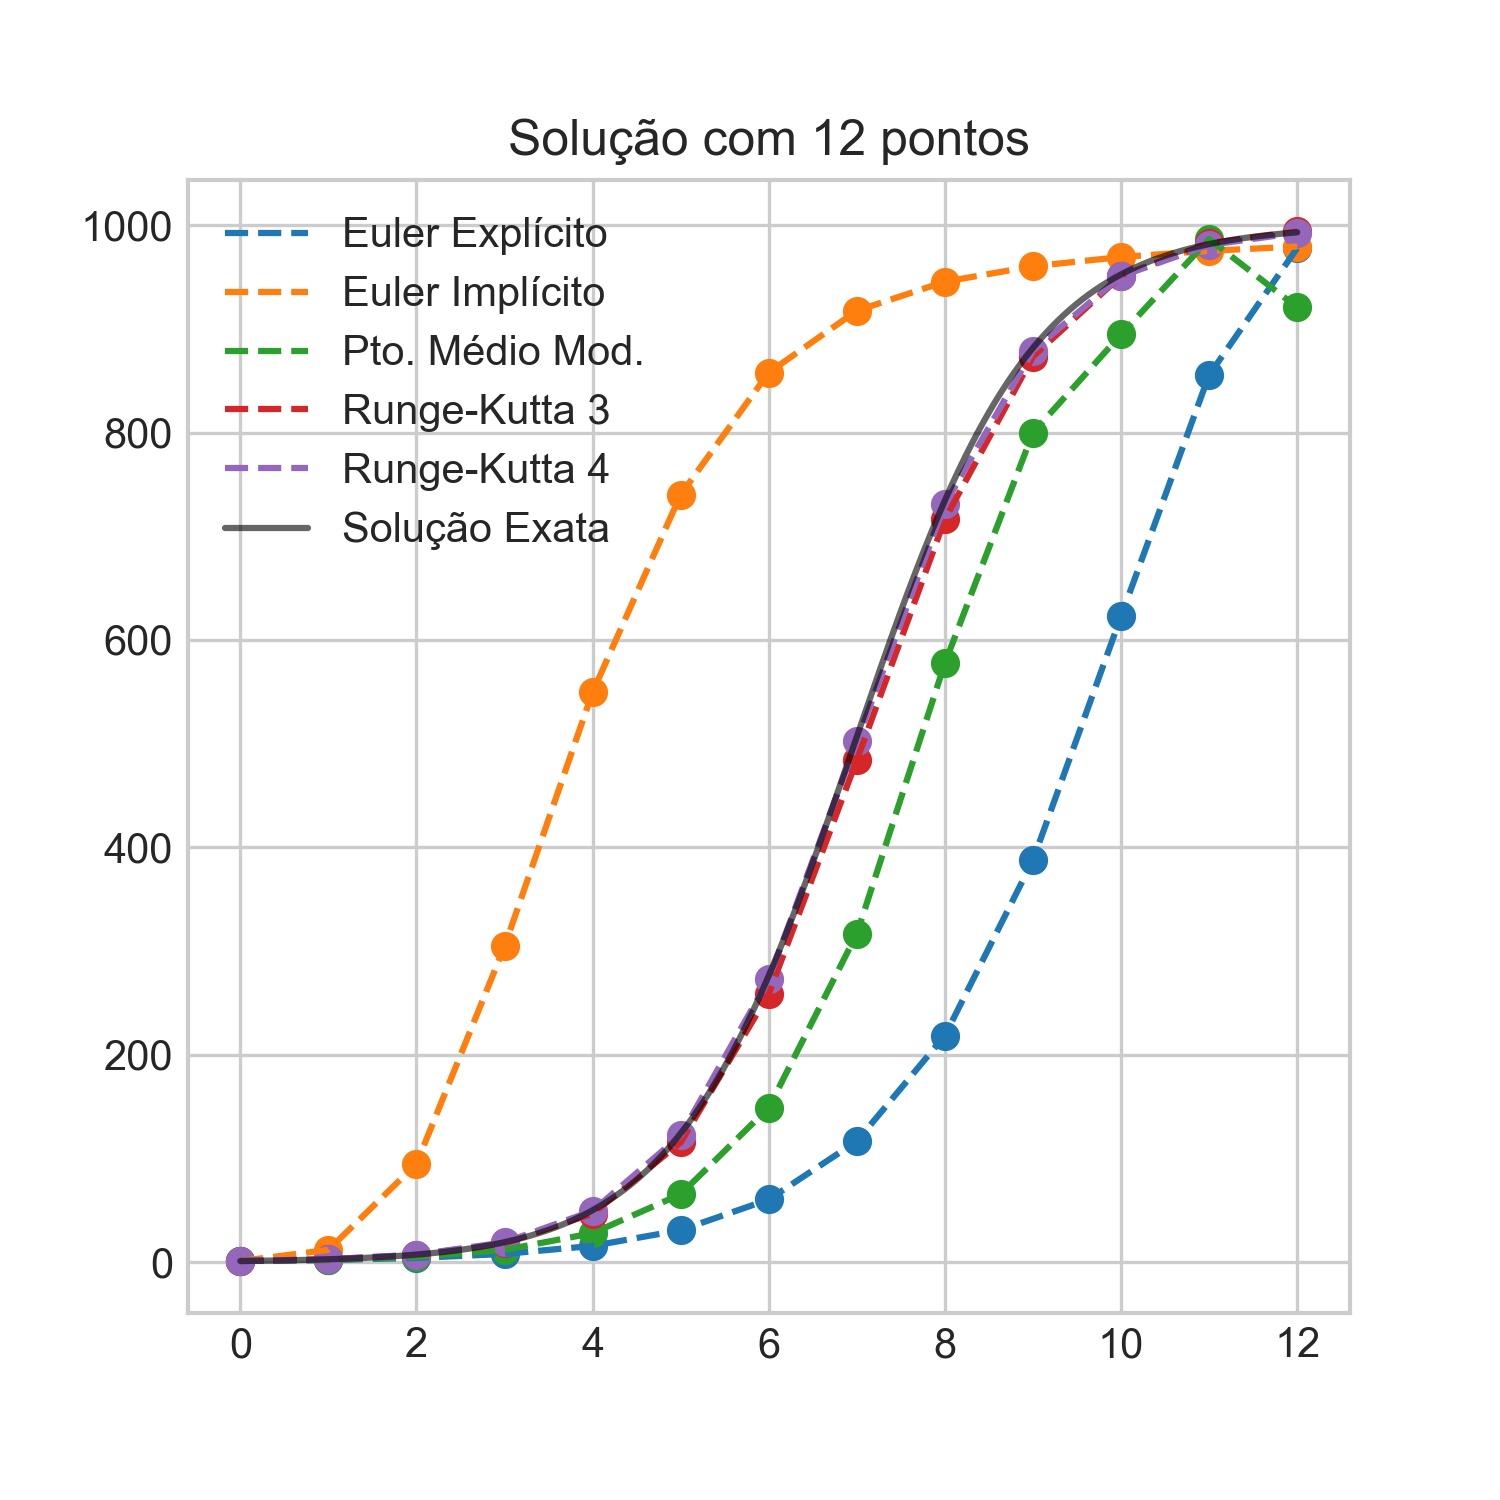
\includegraphics[height=7.8cm, width=7.8cm]{disease/solution_12.png}}
		\subfigure[]{
			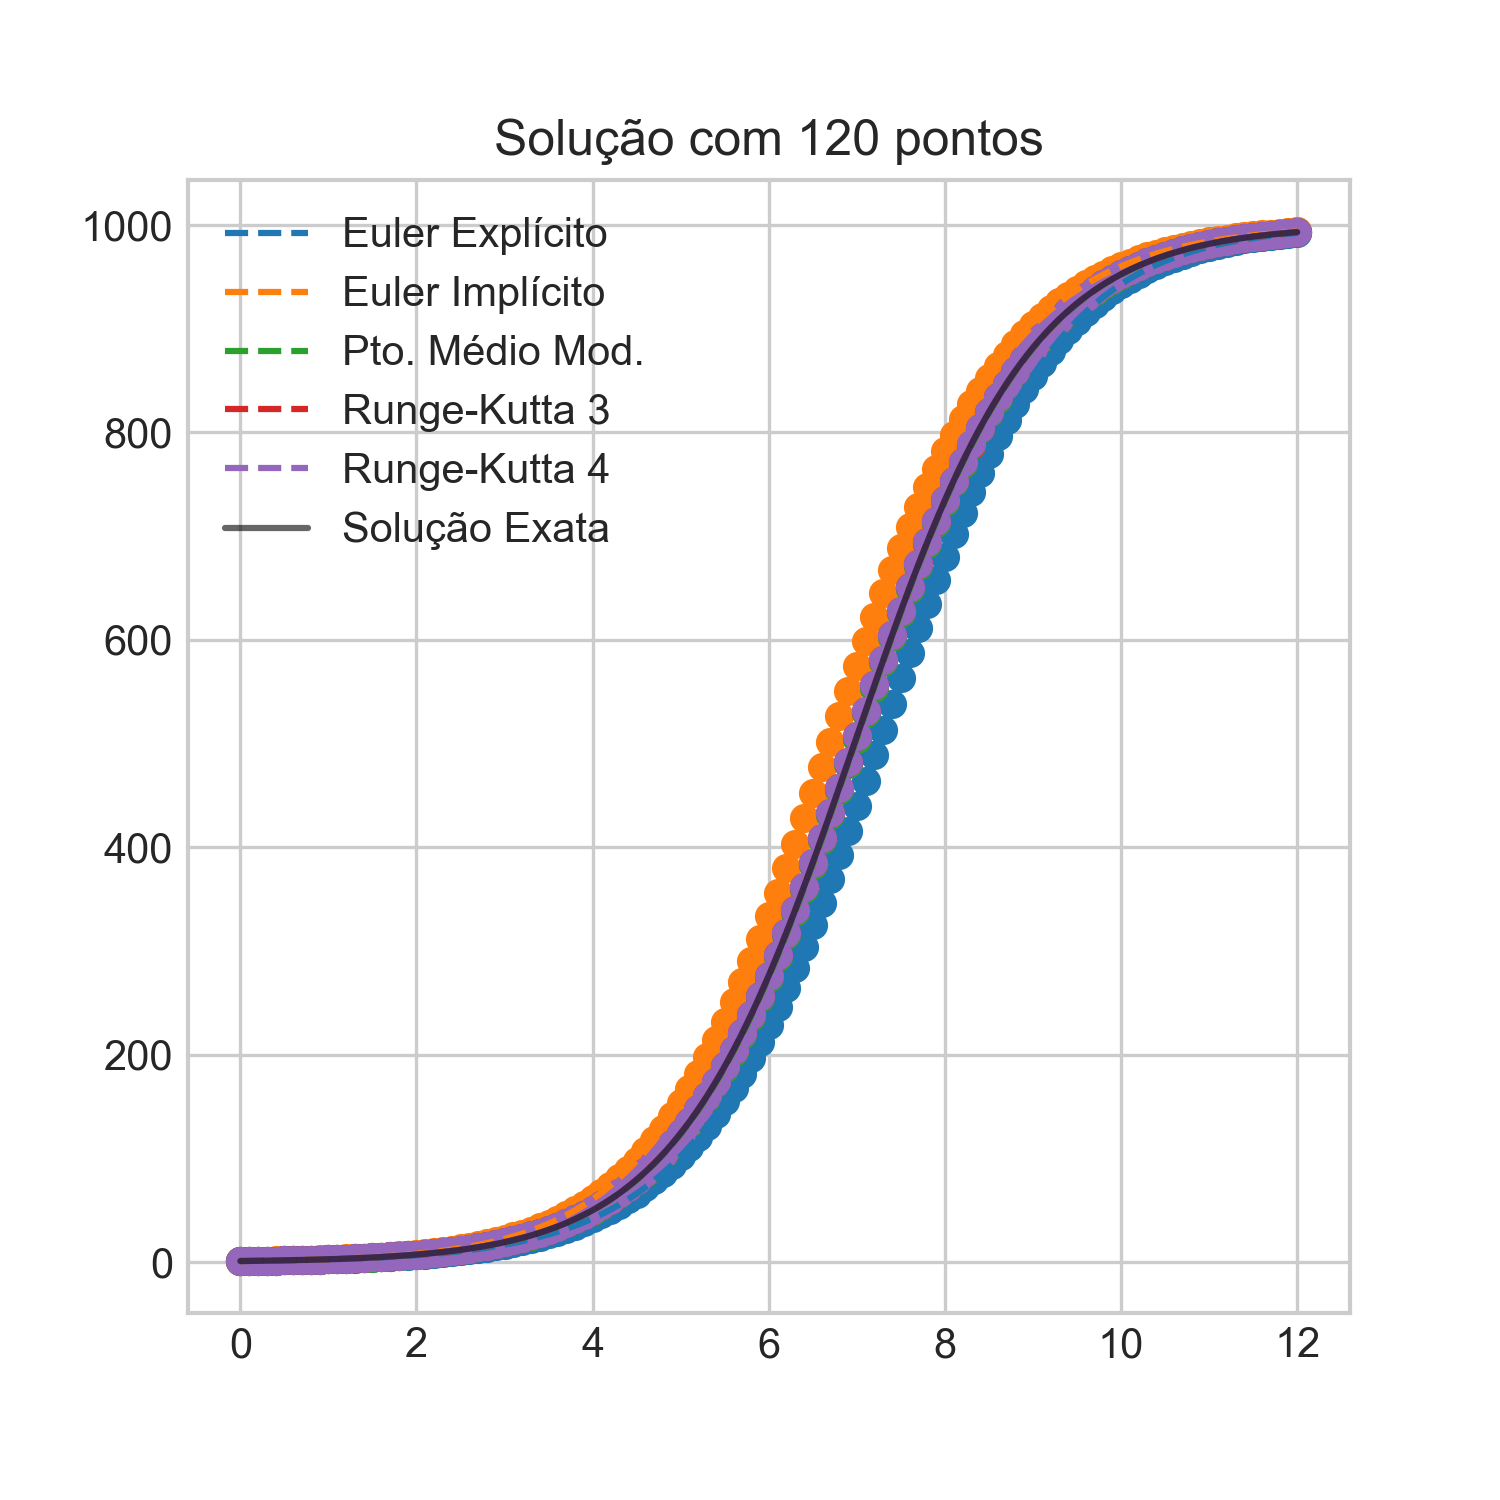
\includegraphics[height=7.8cm, width=7.8cm]{disease/solution_120.png}}
	}
	\mbox{
		\subfigure[]{
			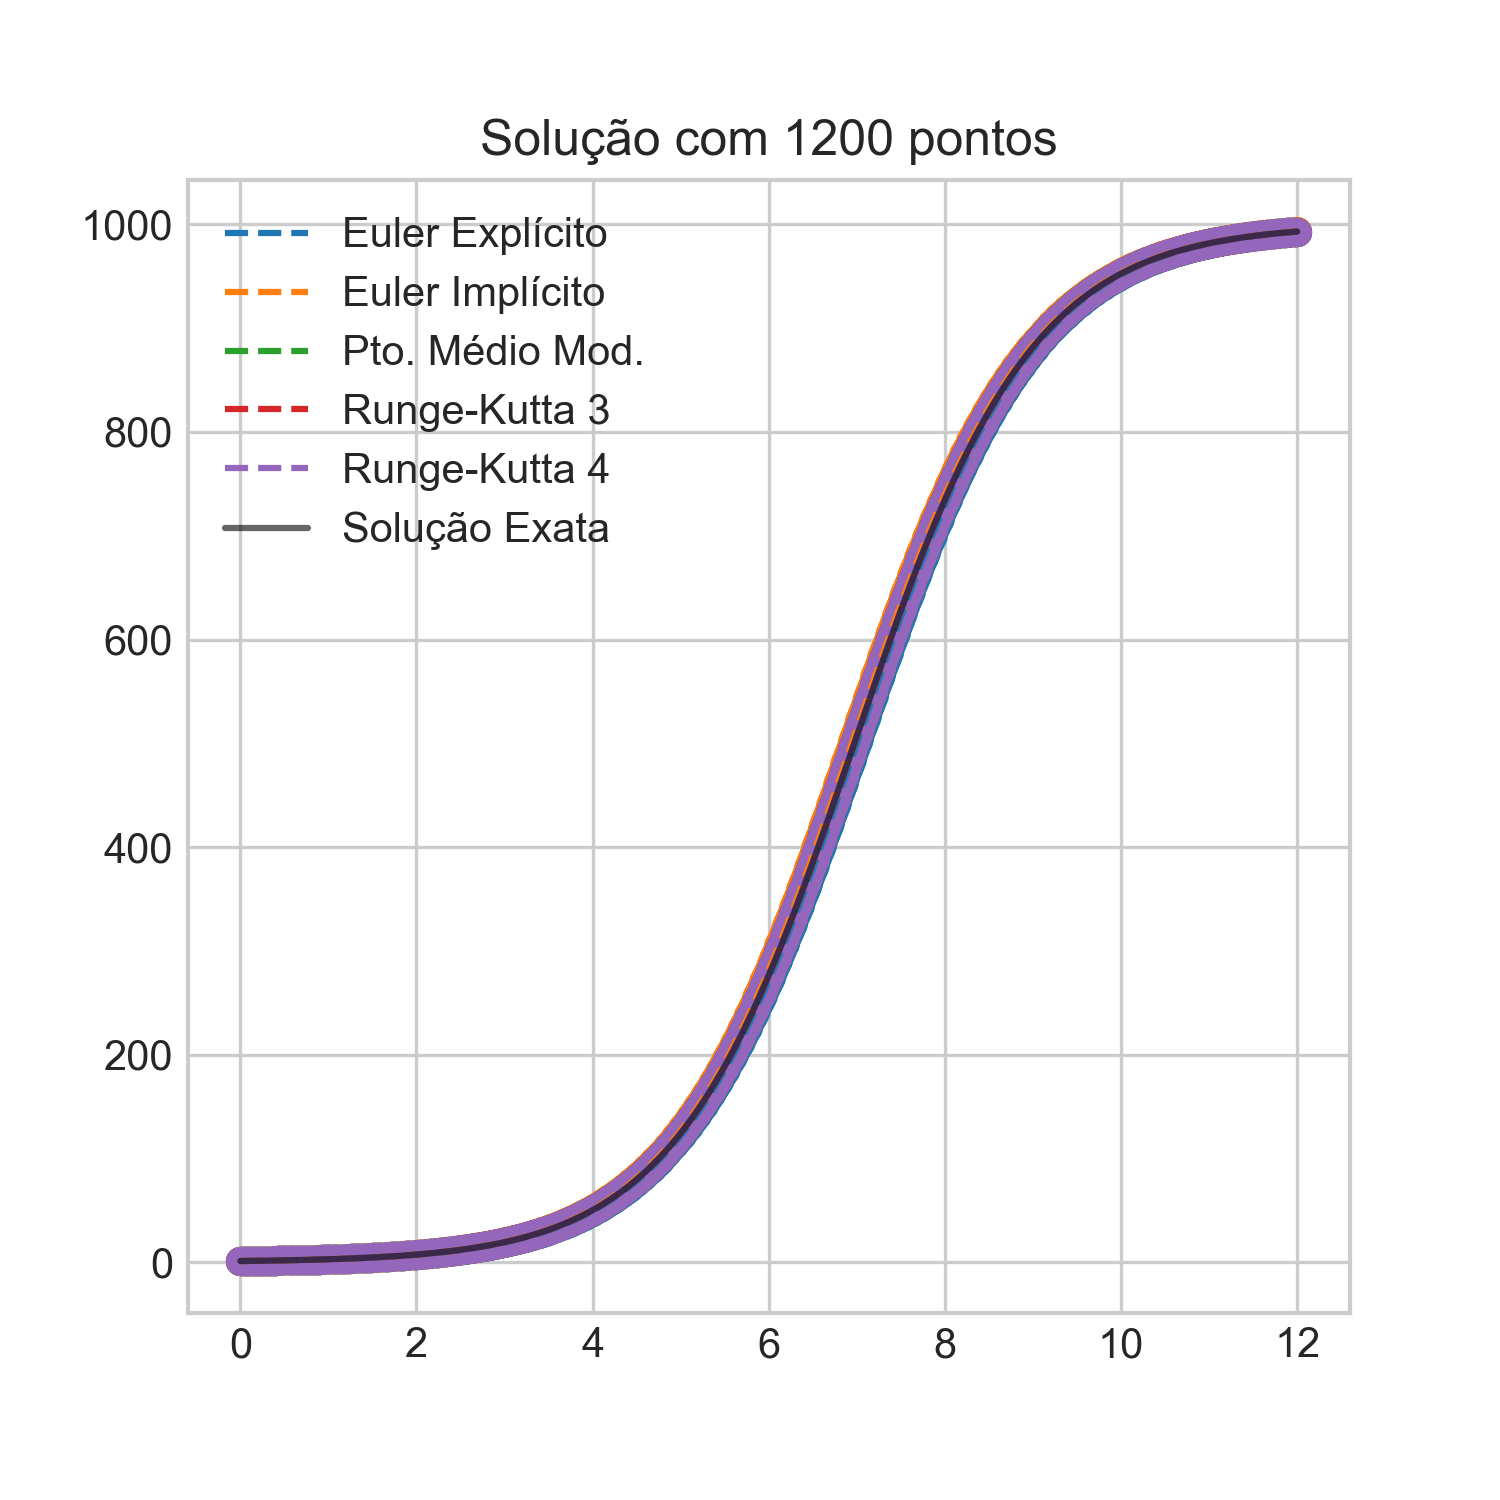
\includegraphics[height=7.8cm, width=7.8cm]{disease/solution_1200.png}}
		\subfigure[]{
			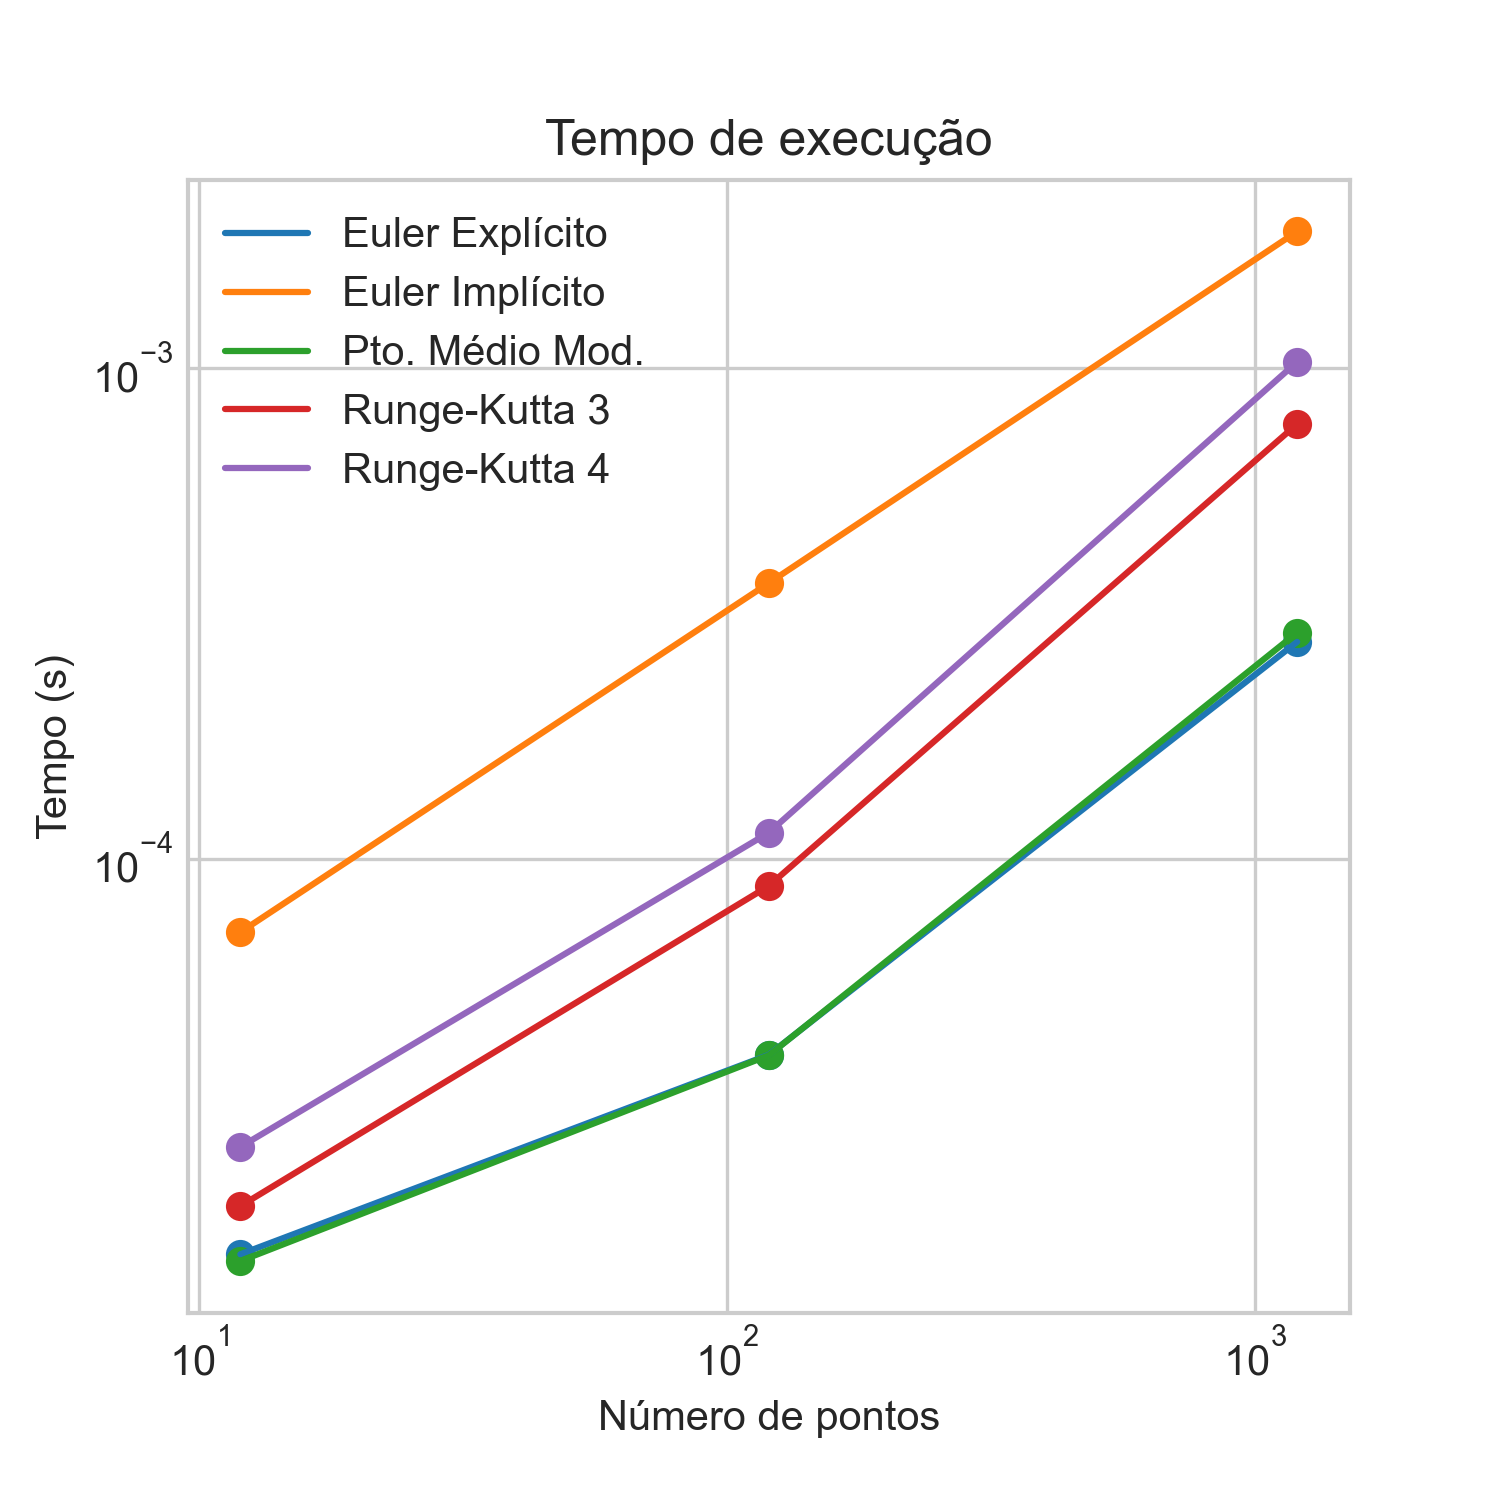
\includegraphics[height=7.8cm, width=7.8cm]{disease/timings.png}}
	}
	\caption{(a) Solução com malha grossa; (b) Solução com malha intermediária; (c) Solução com malha fina; (d) Tempos de execução de cada método. }
    \label{img:ex1_plots}
\end{figure}

Pode-se observar que à medida que o tamanho da malha diminui, as soluções se aproximam cada vez mais da solução analítica, resultando em uma redução do erro de aproximação. Além disso, o tempo de execução aumenta proporcionalmente ao número de pontos da malha.

Outra medida útil para avaliar a precisão dos métodos é o erro relativo, definido como $E_{r} = \Bigg|\dfrac{y_i - y(t_i)}{y(t_i)}\Bigg|$ para $y(t_i) \ne 0$. A Tabela \ref{tab:ex1_relative_errors} apresenta o erro relativo médio para cada método em toda a malha.

% TODO: FIX THIS (2023)
\begin{table}\label{tabela-exemplo1}
	\centering
	\begin{tabular}{|c|c|c|c|c|}
		\hline
		Ordem & \backslashbox{Método}{Pontos} & $12$                   & $120$                  & $1200$                 \\
		\hline
        \rule{0pt}{3ex} 
		1&Euler Explícito & $5.03 \times 10^{-1}$ & $8.50 \times 10^{-2}$ & $9.17 \times 10^{-3}$ \\ \rule{0pt}{3ex} 
        1&Euler Implícito & $4.06 \times 10^{+0}$ & $1.02 \times 10^{-1}$ & $9.34 \times 10^{-3}$ \\ \rule{0pt}{3ex} 
        2&Ponto Médio Modificado & $2.57 \times 10^{-1}$ & $4.08 \times 10^{-3}$ & $4.10 \times 10^{-5}$ \\ \rule{0pt}{3ex} 
        3&Runge-Kutta 3 & $3.22 \times 10^{-2}$ & $6.39 \times 10^{-5}$ & $6.85 \times 10^{-8}$ \\ \rule{0pt}{3ex} 
        4&Runge-Kutta 4 & $6.66 \times 10^{-3}$ & $1.32 \times 10^{-6}$ & $1.42 \times 10^{-10}$ \\
		\hline
		
	\end{tabular}
 \caption{Erros relativos dos métodos computacionais aplicados no PVI do Exemplo $1$.}
 \label{tab:ex1_relative_errors}
\end{table}

Nota-se novamente que métodos de maior ordem tendem a convergir mais rapidamente do que os de menor ordem. Além disso, ao reduzir o espaçamento da malha, diminui-se também o erro relativo médio. Por exemplo, ao diminuir o tamanho da malha em uma magnitude de $10^1$, reduziu-se aproximadamente $10^4$ no erro médio do método de Runge-Kutta de quarta ordem. Na Tabela \ref{tab:ex1_effective_order}, pode-se analisar a ordem efetiva de cada método utilizando (\ref{effective_order}).

\begin{table}[H]
    \centering
    \begin{tabular}{|c|c|}
        \hline
        Método & Ordem de acurácia efetiva\\
        \hline \rule{0pt}{2.5ex} 
         Euler Explícito & $1.01812$\\\rule{0pt}{2.5ex} 
         Euler Implícito & $0.98333$\\\rule{0pt}{2.5ex} 
         Ponto Médio Modificado & $2.00104$\\\rule{0pt}{2.5ex} 
         Runge-Kutta 3 & $2.87502$\\\rule{0pt}{2.5ex} 
         Runge-Kutta 4 & $3.99328$\\
         \hline
    \end{tabular}
    \caption{Ordem efetiva dos erros para cada método estudado.}
    \label{tab:ex1_effective_order}
\end{table}



\subsection{Segundo problema: capacidade de carga}\label{problem-2} \quad
O segundo problema são os estudos de Lotka-Volterra sobre a Lei de Crescimento de Populações, que exploram a capacidade de carga de um meio utilizando funções logísticas. O objetivo é determinar o tamanho máximo da população de uma espécie dada a capacidade máxima do ambiente em que vive e outros fatores, como a taxa de crescimento natural e o número atual de indivíduos vivos. Busca-se assim, simular a evolução do número de indivíduos vivos na população utilizando os métodos iterativos.


O problema pode ser descrito matematicamente com:
\begin{equation}\label{carry_equation_to_be_solved}
	\frac{dP}{dt} = \beta \cdot P \cdot \bigg(1 - \frac{P}{K}\bigg)
\end{equation}

onde:\begin{itemize}
\item $P$ é o número de indivíduos vivos; 
\item $\beta$ é a taxa de crescimento da população;
\item $K$ é a capacidade de carga máxima do sistema;
\item $t$ é a variável de tempo, medida em anos;
\end{itemize}

As equações logísticas são conhecidas pela sua forma em S. Seja $P_0$ a população inicial do problema (\ref{carry_equation_to_be_solved}), observa-se que no início do intervalo a população crescerá lentamente, pois há poucos indivíduos para reproduzirem. A partir desse ponto, $P$ crescerá cada vez mais rapidamente até se aproximar do valor de K, momento em que o crescimento diminuirá, uma vez que $\lim_{P\to K} \big(1 - \frac{P}{K}\big) = 0$. A solução geral de um problema de Lei de Crescimento de Populações de Lotka-Volterra é descrita como:
\begin{equation*}
 P(t) = \dfrac{K}{\dfrac{K - P_0}{P_0} \cdot e^{-\beta t} + 1}
\end{equation*}

Para $\beta = 1$, $K = 1000$, $P_0 = 100$ e o intervalo $[0, 12]$, o PVI a ser resolvido é dado por:
\begin{equation}\label{pvi_carrying-capacity}
    \begin{cases}
	\dfrac{dP}{dt} = \cdot P \cdot \bigg(1 - \dfrac{P}{1000}\bigg) & \\
        P(0) = 100 & t \in [0, 12]
    \end{cases}
\end{equation}
Para este problema, a solução analítica é apresentada como:
\begin{equation*}
    P(t) = \dfrac{3000}{\dfrac{3000 - 100}{100} \cdot e^{-t} + 1} = \dfrac{3000}{29e^{-t} + 1}
\end{equation*}
Utilizando os métodos estudados, a solução numérica obitida para o problema (\ref{pvi_carrying-capacity}) é ilustrada na Figura \ref{img:carry_plots}.
\begin{figure}[H]
	\centering
	\mbox{
		\subfigure[]{
			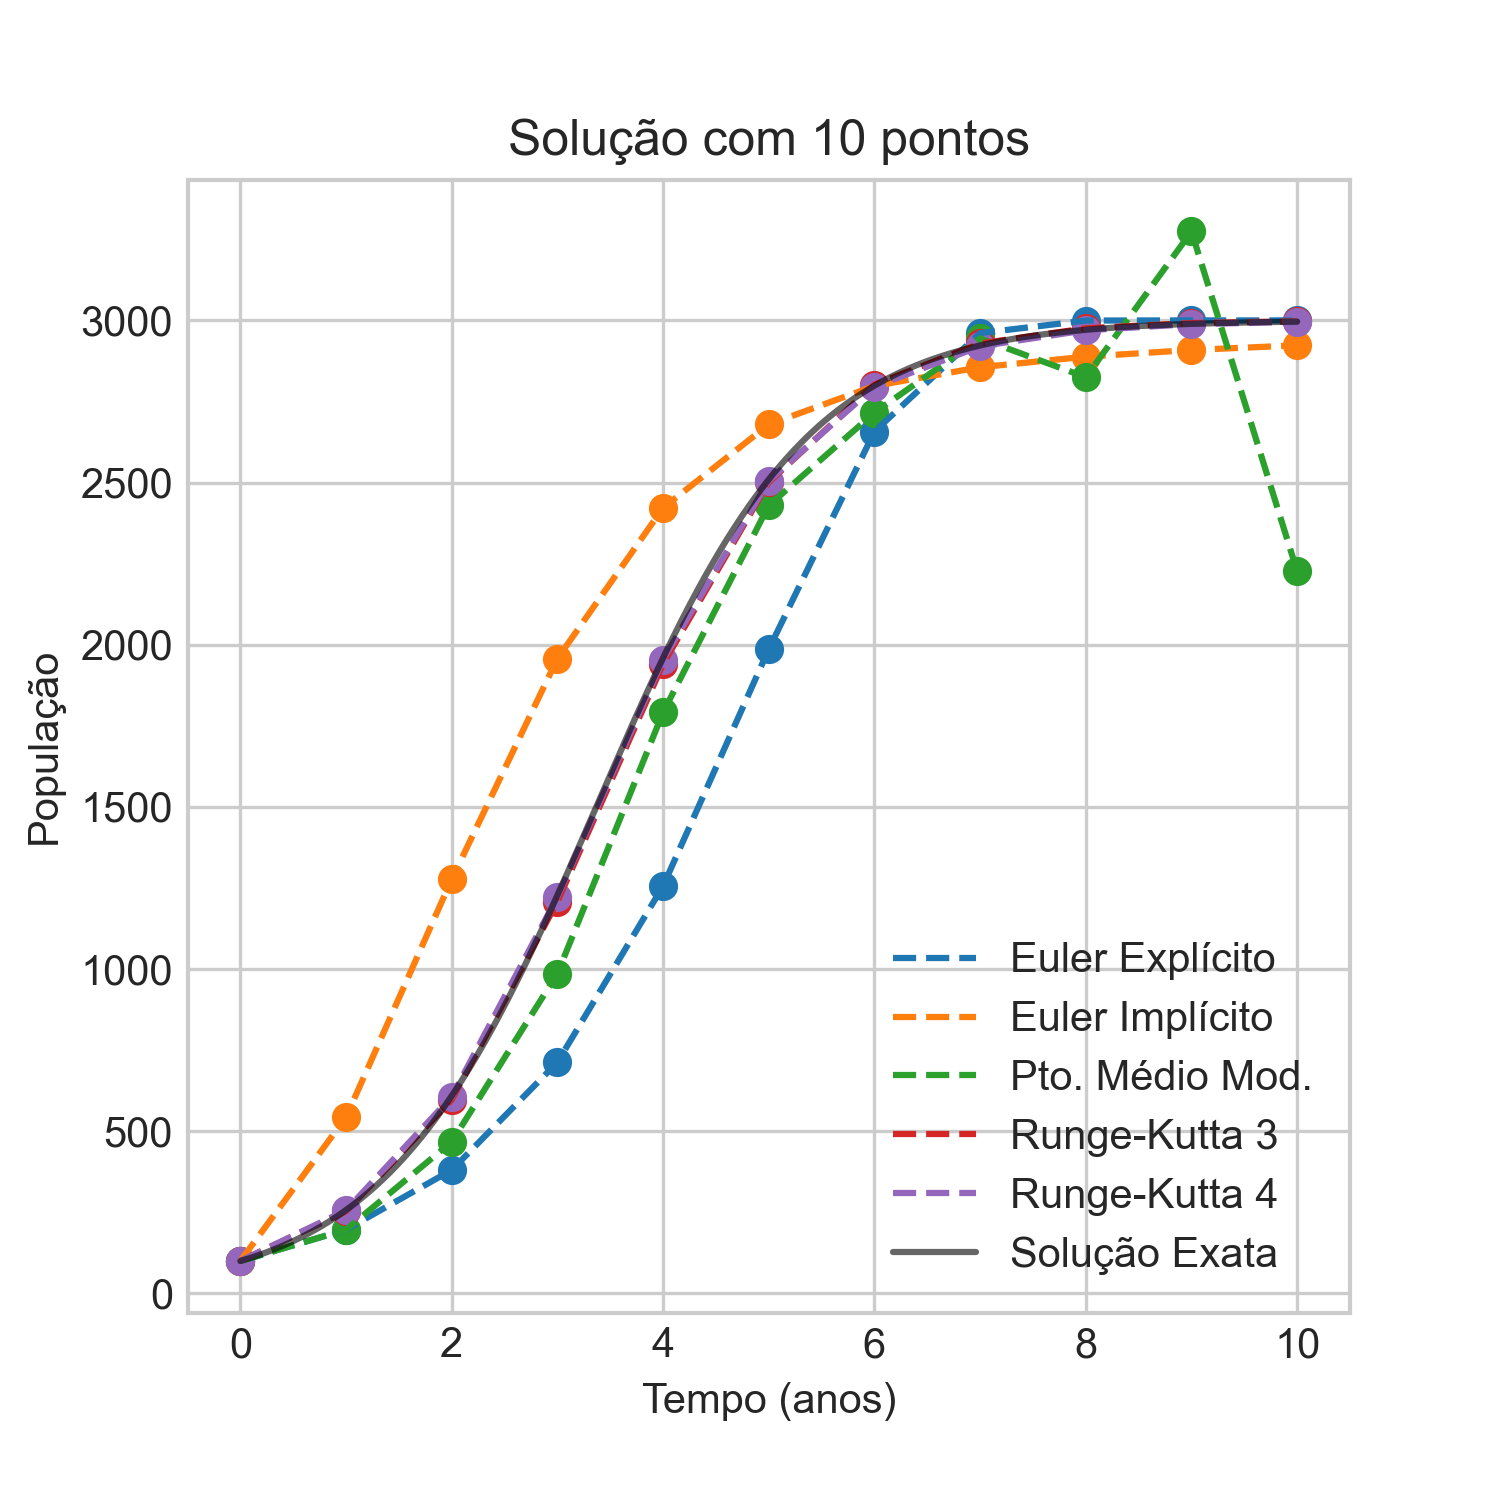
\includegraphics[height=7.8cm, width=7.8cm]{carry-capacity/carry-solution_10_300dpi.png}}
		\subfigure[]{
			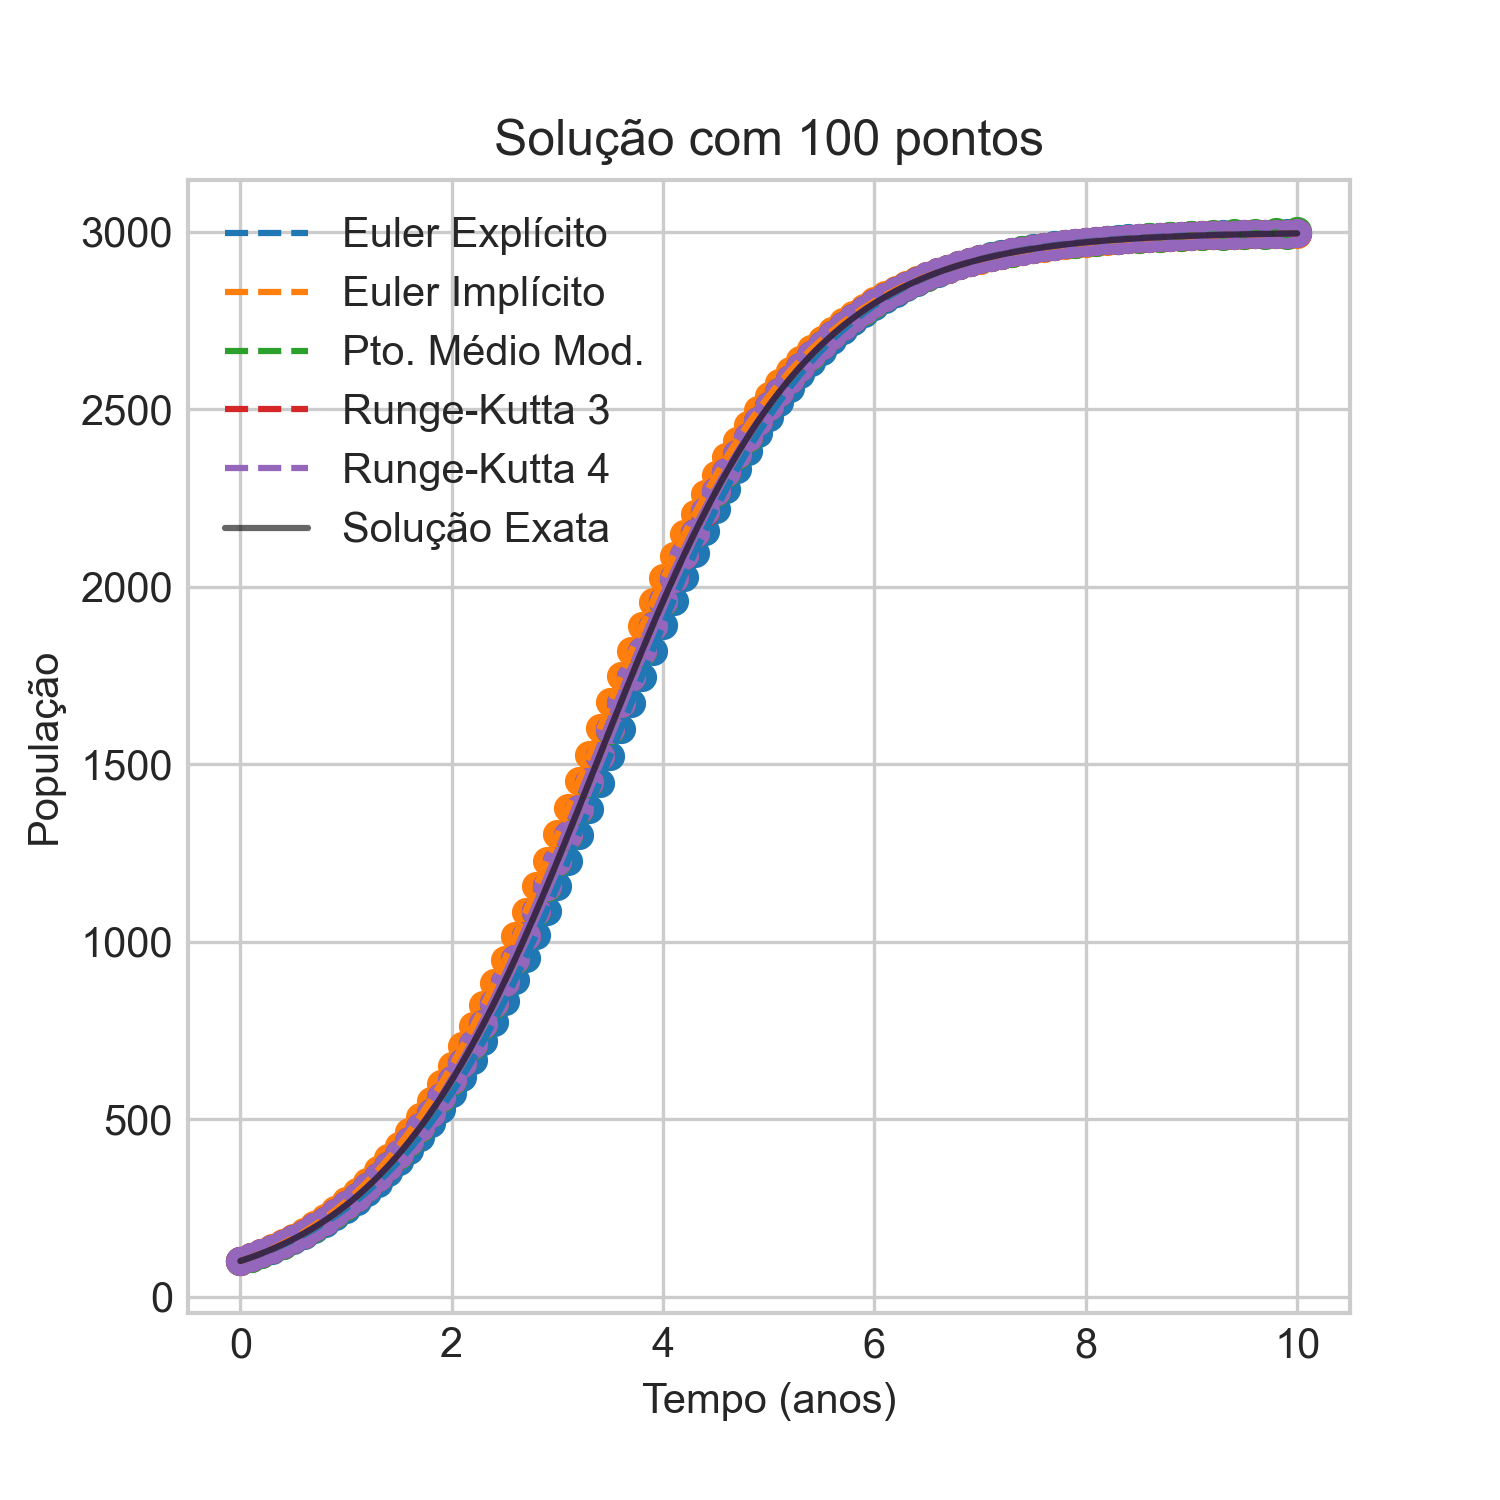
\includegraphics[height=7.8cm, width=7.8cm]{carry-capacity/carry-solution_100_300dpi.png}}
	}
	\mbox{
		\subfigure[]{
			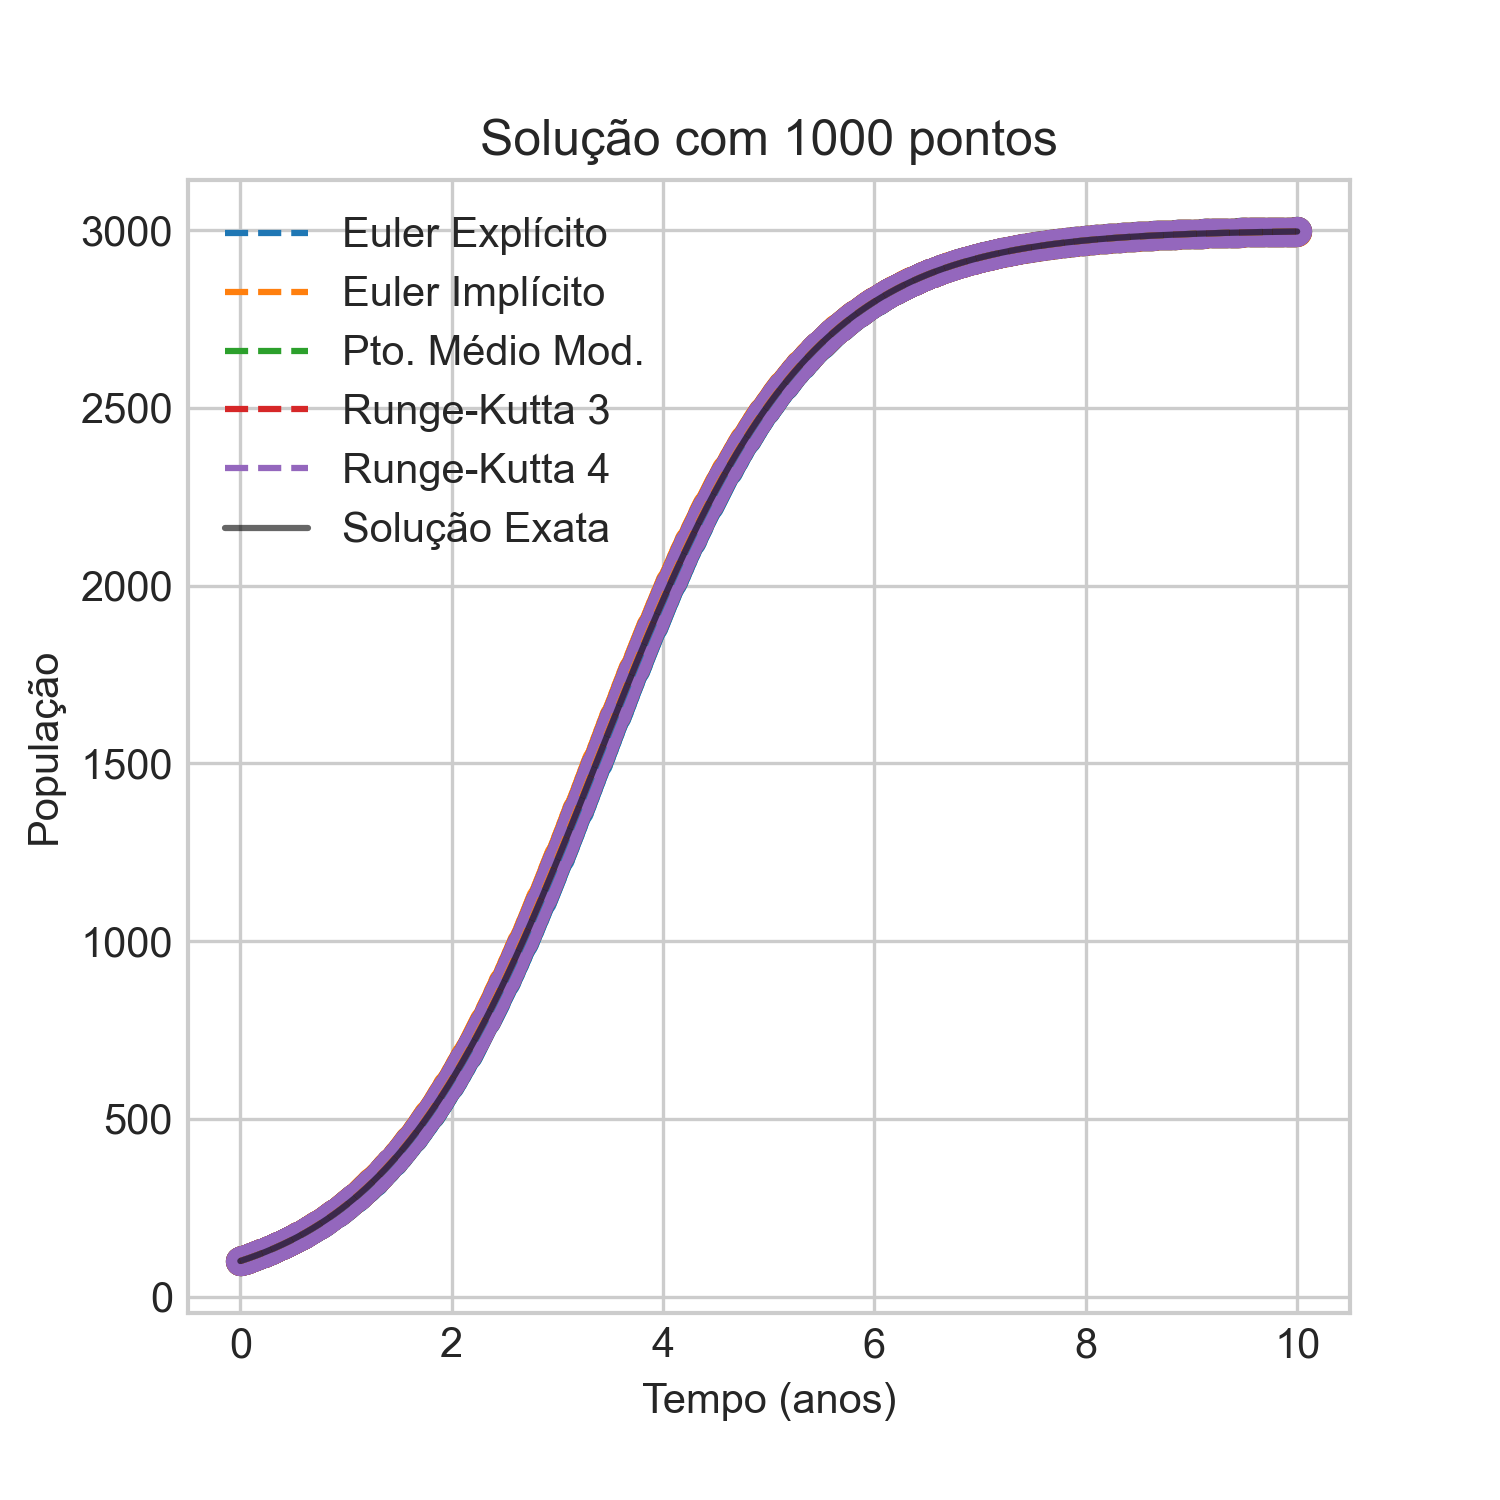
\includegraphics[height=7.8cm, width=7.8cm]{carry-capacity/carry-solution_1000_300dpi.png}}
		\subfigure[]{
			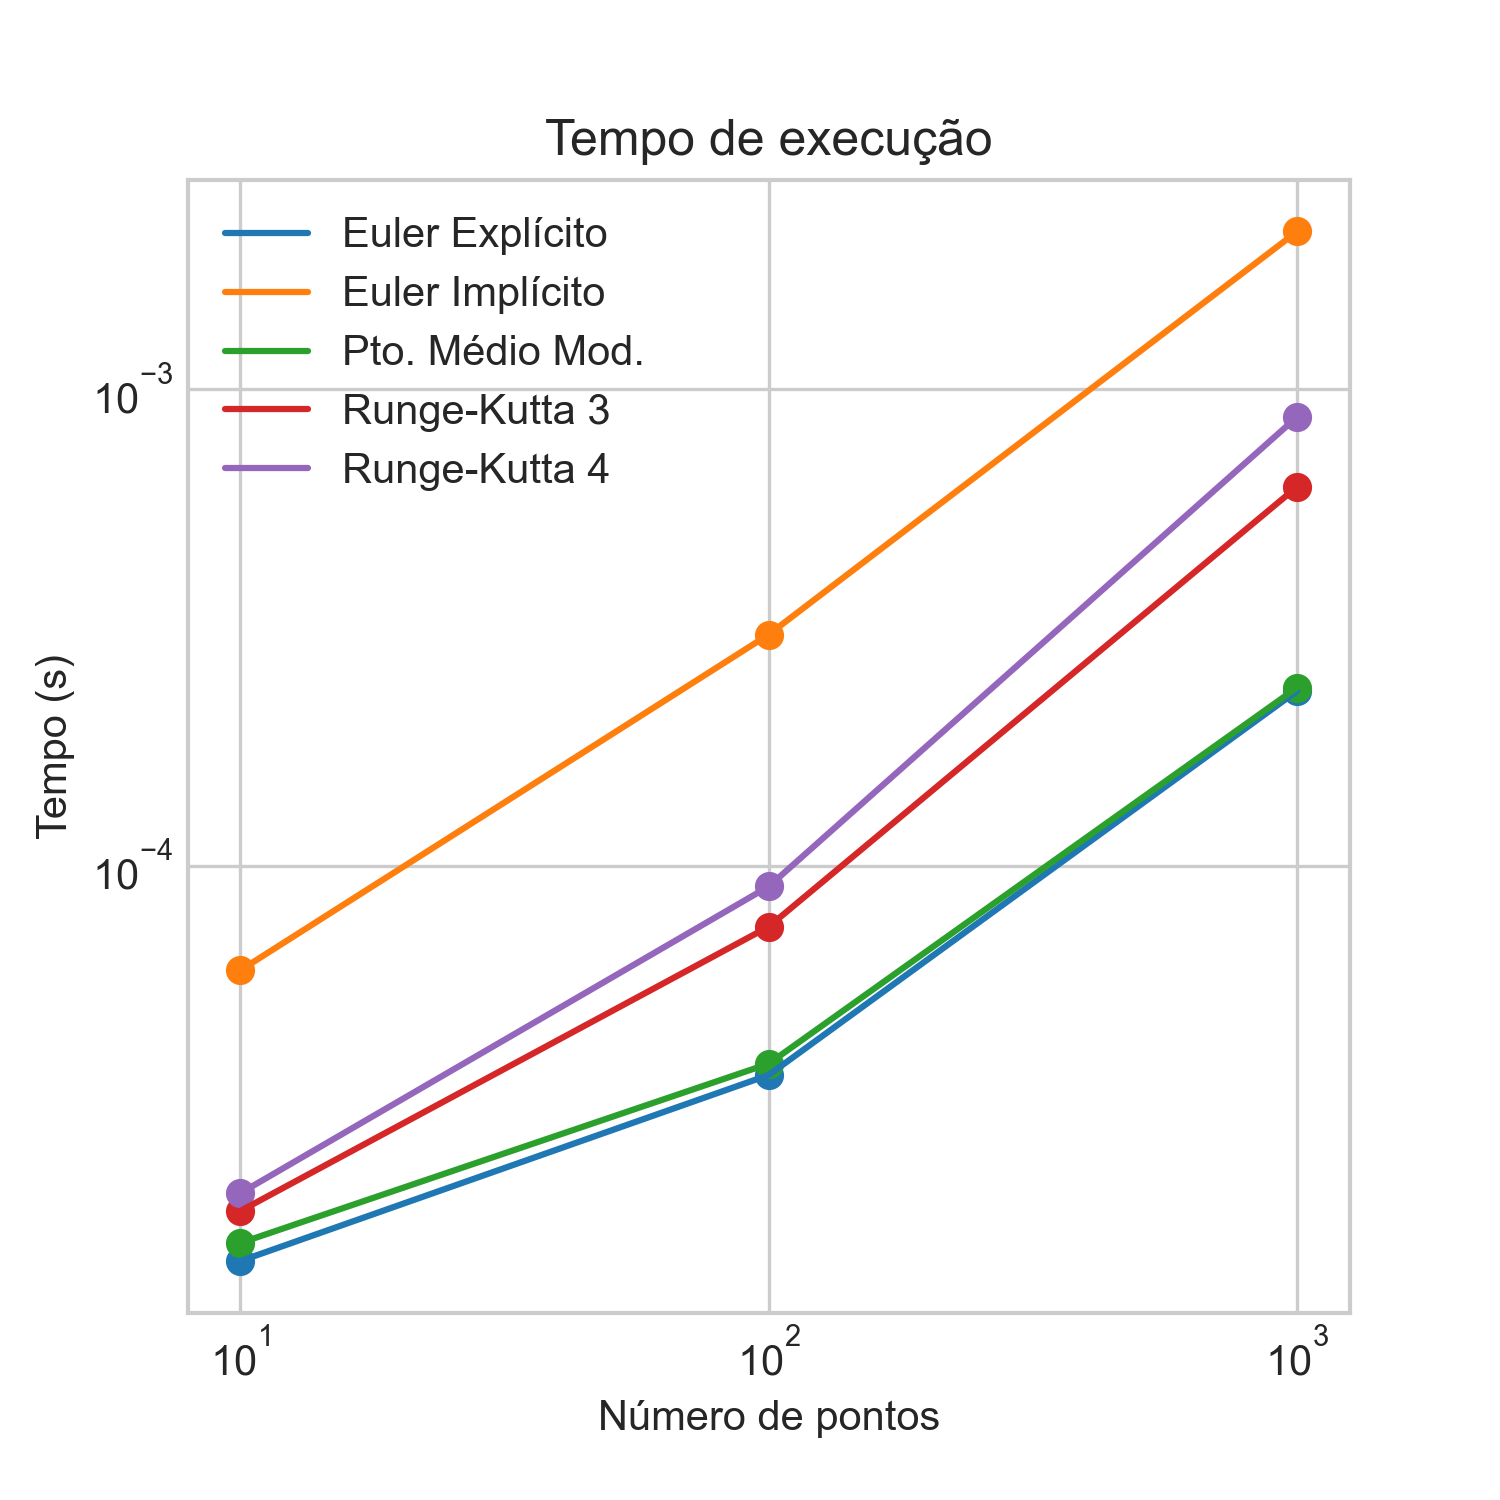
\includegraphics[height=7.8cm, width=7.8cm]{carry-capacity/timings-300dpi.png}}
	}
	\caption{(a) Solução com malha grossa; (b) Solução com malha intermediária; (c) Solução com malha fina; (d) Tempos de execução de cada método. }
    \label{img:carry_plots}
\end{figure}

Assim como no primeiro problema, ao reduzir o tamanho da malha, as soluções convergem para a solução analítica. O erro relativo médio, para cada método, está descrito na Tabela \ref{tab:carry_relative_errors}.

% TODO: Fix this (2023)
\begin{table}\label{tabela-carry}
	\centering
	\begin{tabular}{|c|c|c|c|c|}
		\hline
		Ordem & \backslashbox{Método}{Pontos} & $10$                   & $100$                  & $1000$                 \\
		\hline
        \rule{0pt}{3ex} 
		1&Euler Explícito & $1.67 \times 10^{-1}$ & $2.11 \times 10^{-2}$ & $2.17 \times 10^{-3}$ \\ \rule{0pt}{3ex}
        1&Euler Implícito & $3.19 \times 10^{-1}$ & $2.25 \times 10^{-2}$ & $2.18 \times 10^{-3}$ \\ \rule{0pt}{3ex}
        2&Ponto Médio Modificado & $9.64 \times 10^{-2}$ & $1.30 \times 10^{-3}$ & $1.31 \times 10^{-5}$ \\ \rule{0pt}{3ex}
        3&Runge-Kutta 3 & $6.65 \times 10^{-3}$ & $1.14 \times 10^{-5}$ & $1.21 \times 10^{-8}$ \\ \rule{0pt}{3ex}
        4&Runge-Kutta 4 & $1.76 \times 10^{-3}$ & $2.89 \times 10^{-7}$ & $3.05 \times 10^{-11}$ \\
		\hline
		
	\end{tabular}
 \caption{Erros relativos dos métodos computacionais aplicados no PVI do Exemplo $1$.}
 \label{tab:carry_relative_errors}
\end{table}

Observa-se novamente que os métodos de maior ordem tendem a convergir mais rapidamente do que os métodos de menor ordem. Além disso, ao diminuir o espaçamento da malha, foi possível reduzir o erro relativo médio: por exemplo, ao reduzir o tamanho da malha em uma ordem de magnitude ($10^1$), obteve-se uma redução no erro médio de cada método na ordem de $10^{O(h)}$. Vale ressaltar que a ordem efetiva de cada método pode ser analisada na Tabela \ref{tab:carry_effective_order}, utilizando a equação (\ref{effective_order}).

\begin{table}[H]
    \centering
    \begin{tabular}{|c|c|}
        \hline
        Método & Ordem de acurácia efetiva\\
        \hline \rule{0pt}{2.5ex} 
        Euler Explícito & 0.99593\\\rule{0pt}{2.5ex} 
        Euler Implícito & 1.00228\\\rule{0pt}{2.5ex} 
        Ponto Médio Modificado & 1.99196\\\rule{0pt}{2.5ex} 
        Runge-Kutta 3 & 3.04741\\\rule{0pt}{2.5ex} 
        Runge-Kutta 4 & 4.01748\\
         \hline
    \end{tabular}
    \caption{Ordem efetiva dos erros para cada método estudado.}
    \label{tab:carry_effective_order}
\end{table}

Por fim, embora a estabilidade dos métodos utilizados não tenha sido abordada neste trabalho, vale ressaltar que em ambos os exemplos o método do Ponto Médio Modificado (uma adaptação das diferenças centradas) apresentou instabilidade em sua solução, sendo mais evidente em malhas mais grossas. Embora o método do Ponto Médio Modificado seja de ordem superior ao método de Euler Explícito, mantendo um custo computacional semelhante, como pode ser visto nas Figuras $\ref{img:ex1_plots}d$ e $\ref{img:carry_plots}d$, está mais sujeito a instabilidade numérica e requer condições mais restritas de espaçamento de malha \cite{ascher2008numerical}.

%%%%%%%%%%%%%%%%%%%%%%%%%%%%%%%%%%%%%%%%%%%%%%%%
\subsection{Terceiro problema: populações de predadores e presas}\label{problem-3} \quad
O terceiro problema consiste em uma equação competitiva de Lotka-Volterra \cite{goel1971} que modela a dinâmica de populações de predadores e presas. Esse modelo considera duas populações, uma de predadores $A$ e outra de presas $B$, tal que:

\emph{
	No início de um período, as presas se reproduzem e, ao final do período, cada indivíduo em média produz $r$ filhos. As presas não morrem naturalmente, mas estão sujeitas a serem predadas com uma probabilidade $p$. Por outro lado, os predadores morrem rapidamente de fome e, se não são alimentados, morrem na proporção $s$. A taxa de reprodução dos predadores está relacionada à sua capacidade de alimentação, que depende da quantidade de presas vivas.}". Adaptado de \cite{burkardt2009}.

O problema em questão é descrito matematicamente por um sistema de equações diferenciais ordinárias, dado por:

\begin{equation*}\label{predator_formula}
	\dfrac{dA}{dt} = r_AAB - sA
\end{equation*}

\begin{equation*}\label{prey_formula}
	\dfrac{dB}{dt} = r_BB - pAB
\end{equation*}

onde:

\begin{itemize}
\item $A$ é o número de predadores vivos;
\item $B$ é o número de presas vivas;
\item $r_A$ é a taxa de crescimento da população de predadores;
\item $r_B$ é a taxa de crescimento da população de presas;
\item $p$ é a probabilidade de uma presa ser capturada e morta por um predador;
\item $s$ é a proporção de predadores que morrem de fome;
\item $t$ é a variável temporal, medida em anos.
\end{itemize}

Considerando as populações iniciais $A_0 = 100$ e $B_0 = 4000$, e os valores dos parâmetros $r_A = 3 \times 10^{-3}$, $r_B = 3$, $p = 1 \times 10^{-2}$ e $s = 10$, obtêm-se o seguinte problema de valor inicial (PVI):

\begin{equation}\label{pvi-predator-prey}
	\begin{cases}
		\dfrac{dA}{dt} = 0.003AB - 10A &                            \\[3mm]
        \dfrac{dB}{dt} = 3B - 0.01AB   &                            \\[2mm]
		A(0) = 100                    &                            \\
        B(0) = 4000                   & \text{ com } t \in [0, 10] 
	\end{cases}
\end{equation}

Para resolver este problema, foram aplicados os métodos de Euler Implícito e Runge-Kutta de 4ª ordem com 500 pontos, visto que ambos geram resultados representativos. Os gráficos das soluções obtidas por estes métodos estão representados nas Figuras \ref{img:explicit_euler_plots} e \ref{img:rk4_plots}.
\begin{figure}[H]
	\centering
	\mbox{
		\subfigure[]{
			\includegraphics[height=8cm, width=8cm]{predator-prey/predator_prey-300dpi-Euler_Implícito-500points-2d.png}}
		\subfigure[]{
			\includegraphics[height=8cm, width=8cm]{predator-prey/predator_prey-300dpi-Euler_Implícito-500points-2d-up.png}}
	}
	\mbox{
		\subfigure[]{
			\includegraphics[height=12cm, width=12cm]{predator-prey/predator_prey-300dpi-Euler_Implícito-500 points.png}}
	}
	\caption{Método de Euler Implícito - (a) Evolução de ambas populações temporalmente; (b) Número de indivíduos vivos simultaneamente em diferentes instantes de tempo; (c) Representação tridimensional da evolução do problema.}
    \label{img:explicit_euler_plots}
\end{figure}

\begin{figure}[H]
	\centering
	\mbox{
		\subfigure[]{
			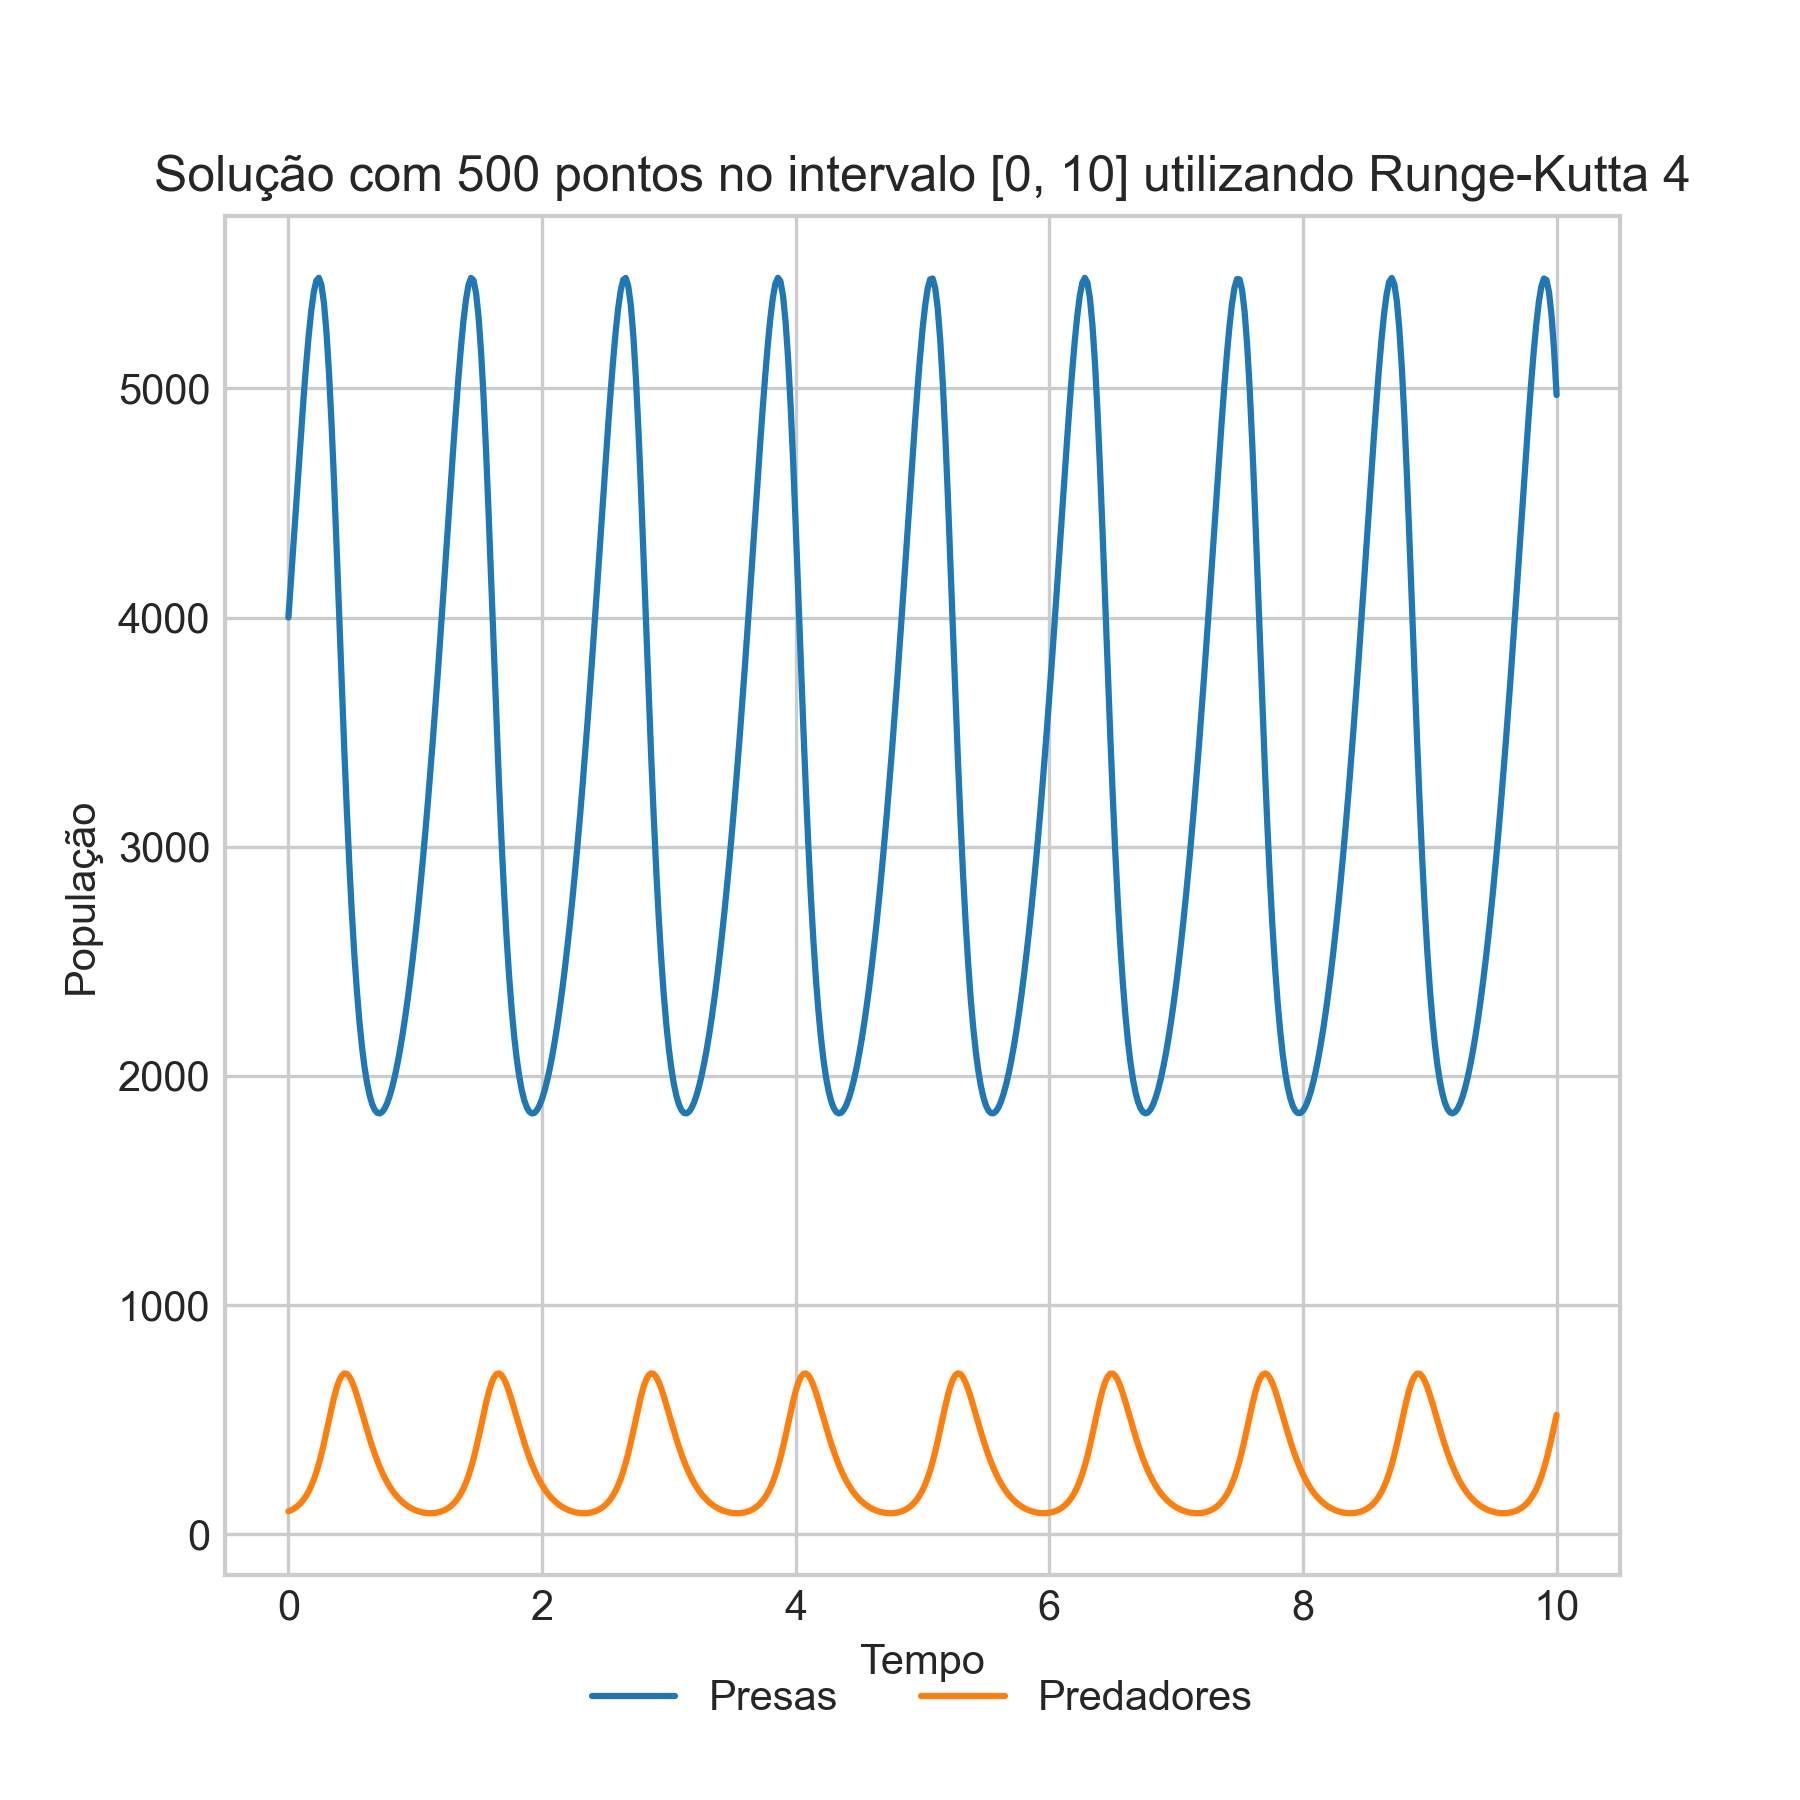
\includegraphics[height=8cm, width=8cm]{predator-prey/predator_prey-300dpi-Runge-Kutta_4-500points-2d.png}}
		\subfigure[]{
			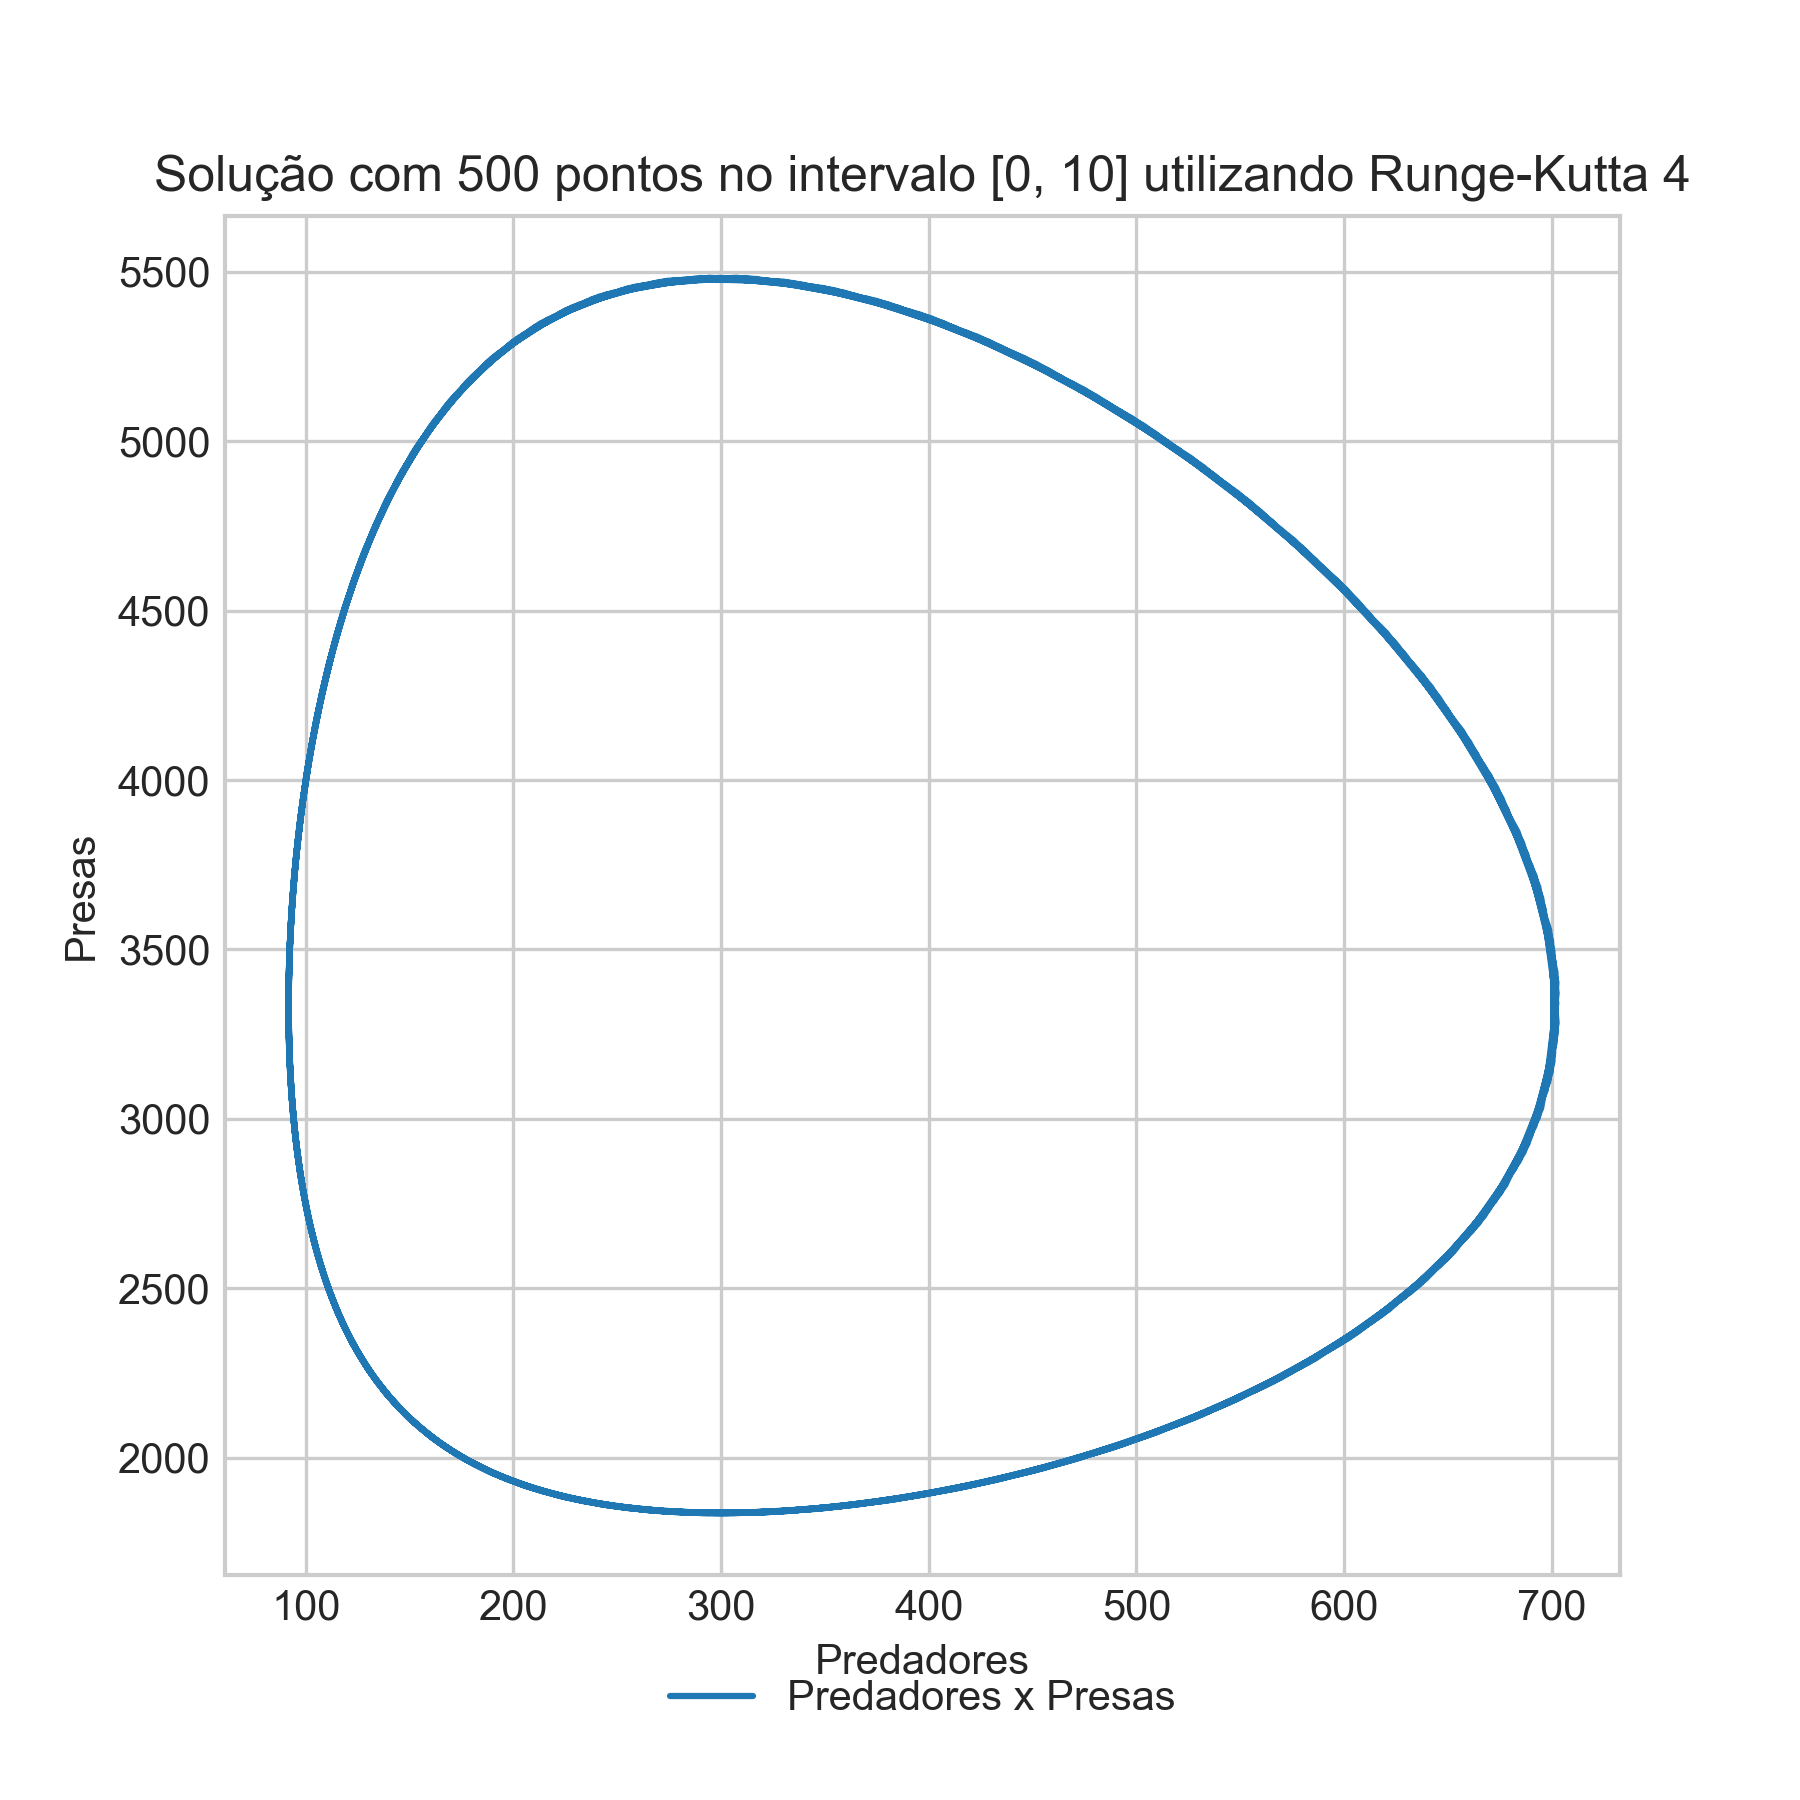
\includegraphics[height=8cm, width=8cm]{predator-prey/predator_prey-300dpi-Runge-Kutta_4-500points-2d-up.png}}
	}
	\mbox{
		\subfigure[]{
			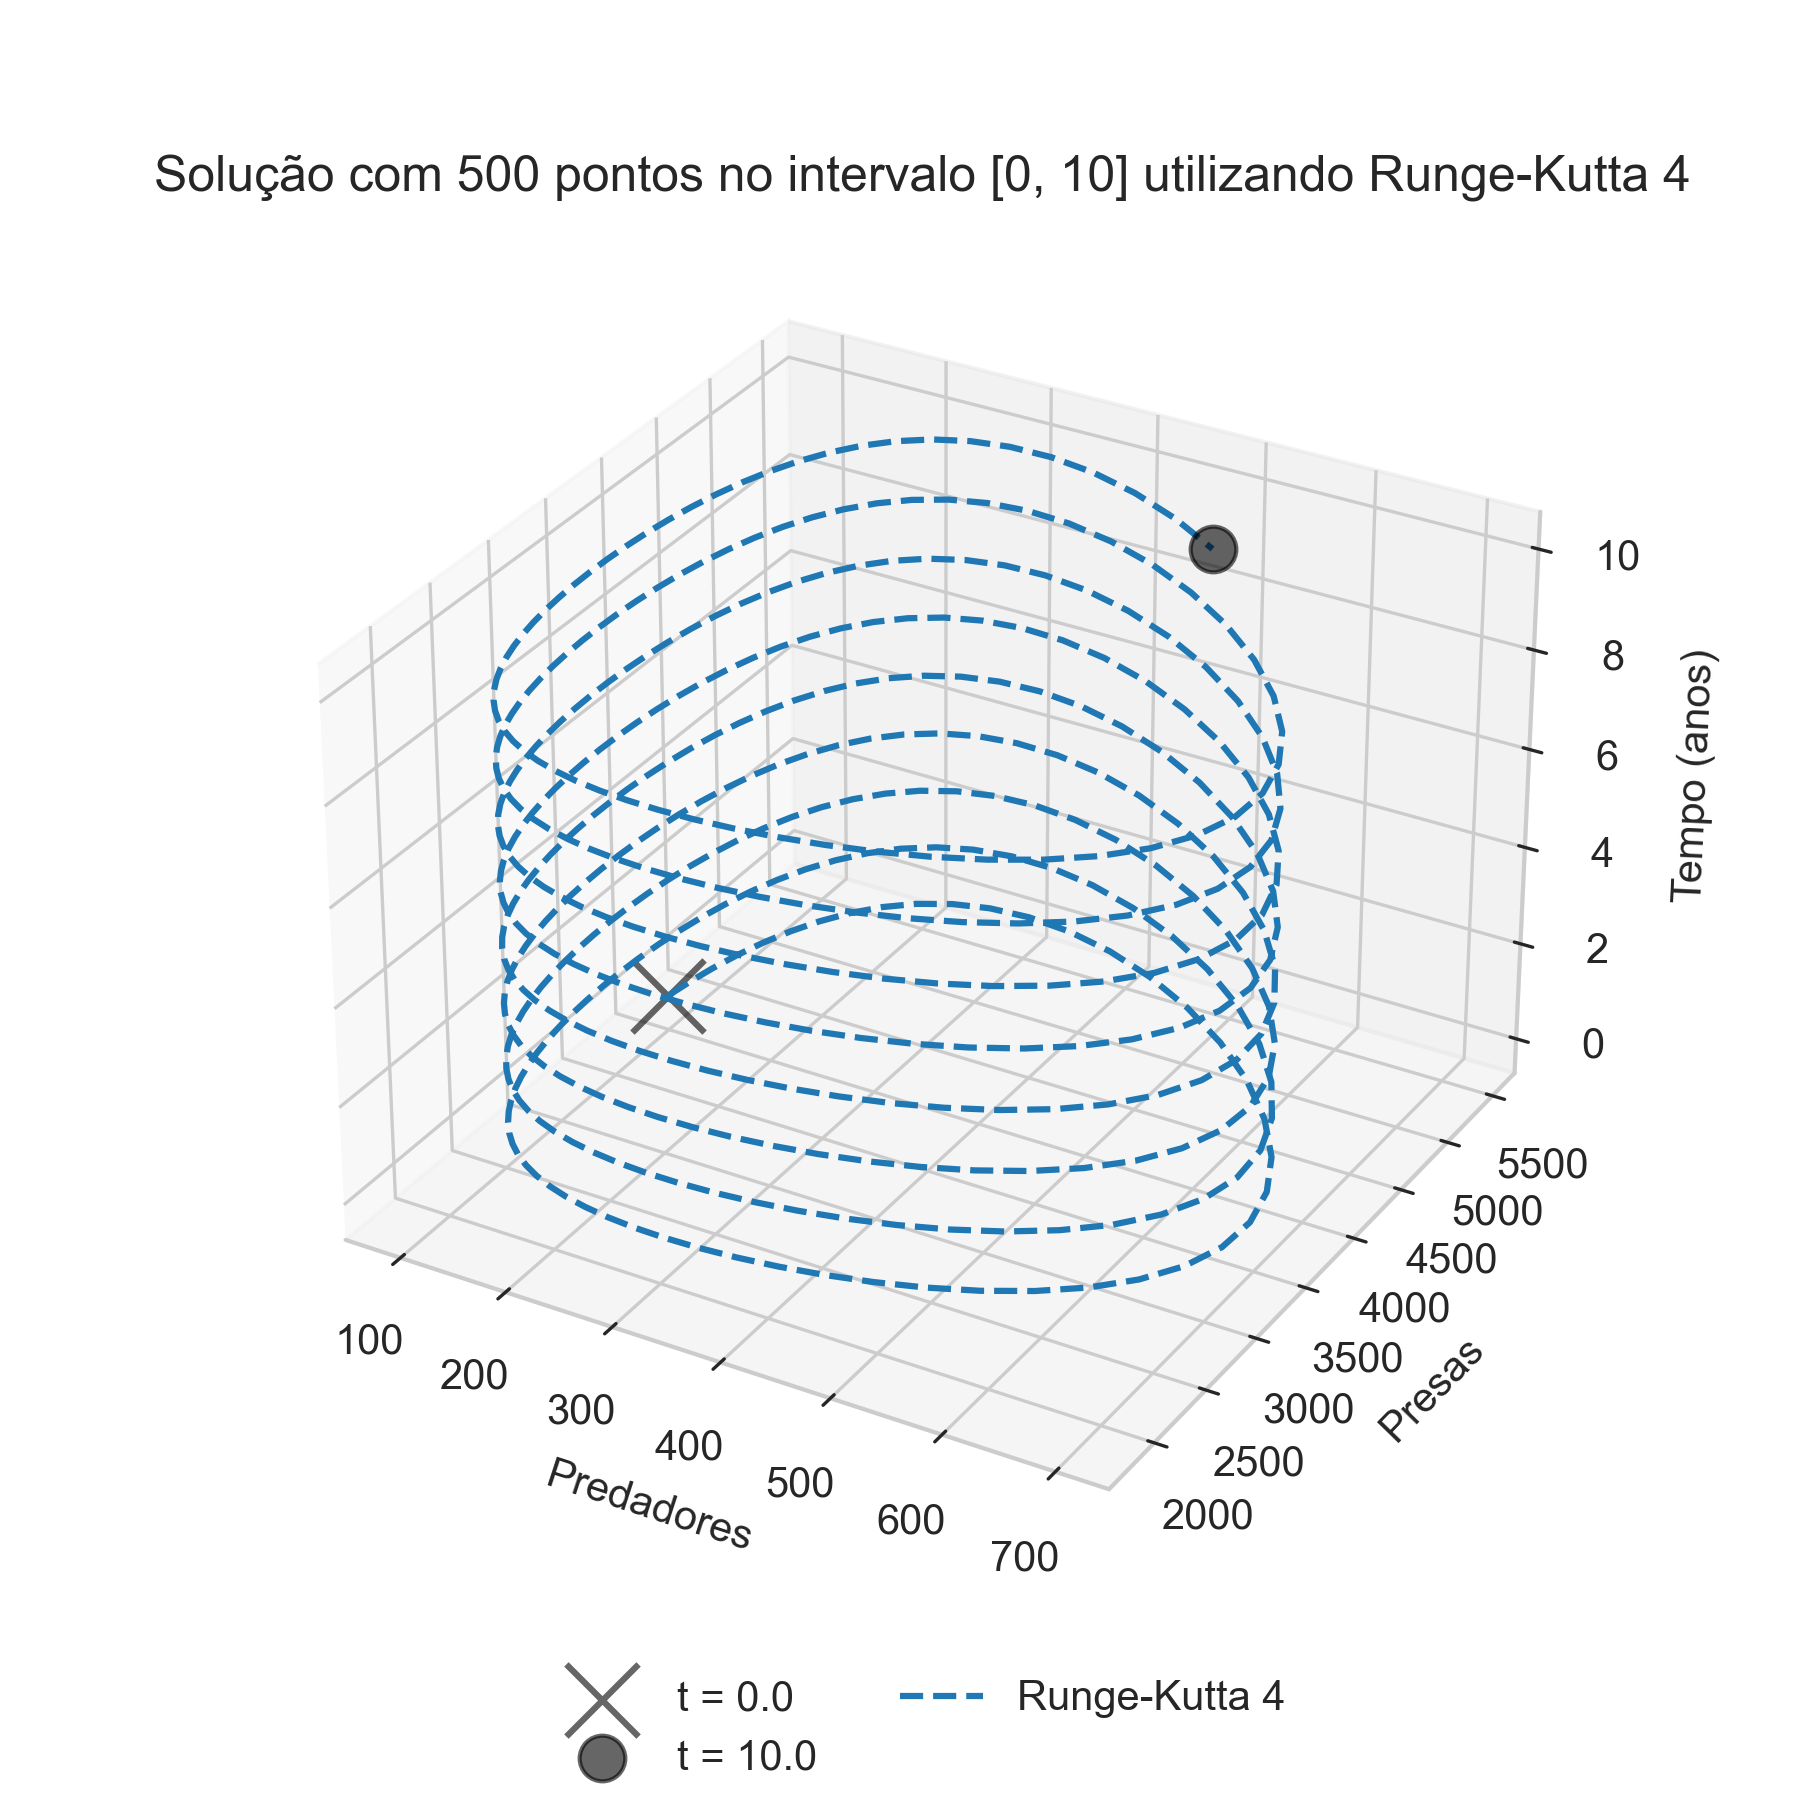
\includegraphics[height=12cm, width=12cm]{predator-prey/predator_prey-300dpi-Runge-Kutta_4-500 points.png}}
	}
	\caption{Método de Runge-Kutta de 4ª ordem - (a) Evolução de ambas populações temporalmente; (b) Número de indivíduos vivos simultaneamente em diferentes instantes de tempo; (c) Representação tridimensional da evolução do problema.}
    \label{img:rk4_plots}
\end{figure}

Constata-se que ambas soluções simulam de forma semelhante a relação de predação, onde a população de predadores cresce quando há muitas presas para se alimentar, assim como a população de presas cresce vertiginosamente quando há poucos predadores e vice-versa.

Na Figura \ref{img:explicit_euler_plots}, é possível observar que o método de Euler Implícito reduz a amplitude dos ciclos das populações ao longo do tempo, resultando em um comportamento espiral. A partir do início do intervalo, cada ano manteve o comportamento da curva, mas reduziu a variação da população. Embora novos indivíduos surjam e outros faleçam, a quantidade de indivíduos vivos simultaneamente tende a um valor constante.

Ao estudar a solução pelo método explícito de quarta ordem, observa-se que na Figura \ref{img:rk4_plots}, forma-se um gráfico periódico, em que cada ano reproduz o anterior identicamente.

Para verificar se os resultados convergem para a solução apropriada do problema, é utilizada a mesma técnica de refinamento de malha aplicada nos problemas (\ref{problem-1}) e (\ref{problem-2}). Essa técnica utiliza uma malha grossa, intermediária e fina para obter resultados cada vez mais precisos. Os resultados são ilustrados na Figura \ref{img:comparison_plots}.

\begin{figure}[H]
	\centering
	\mbox{
		\subfigure[]{
			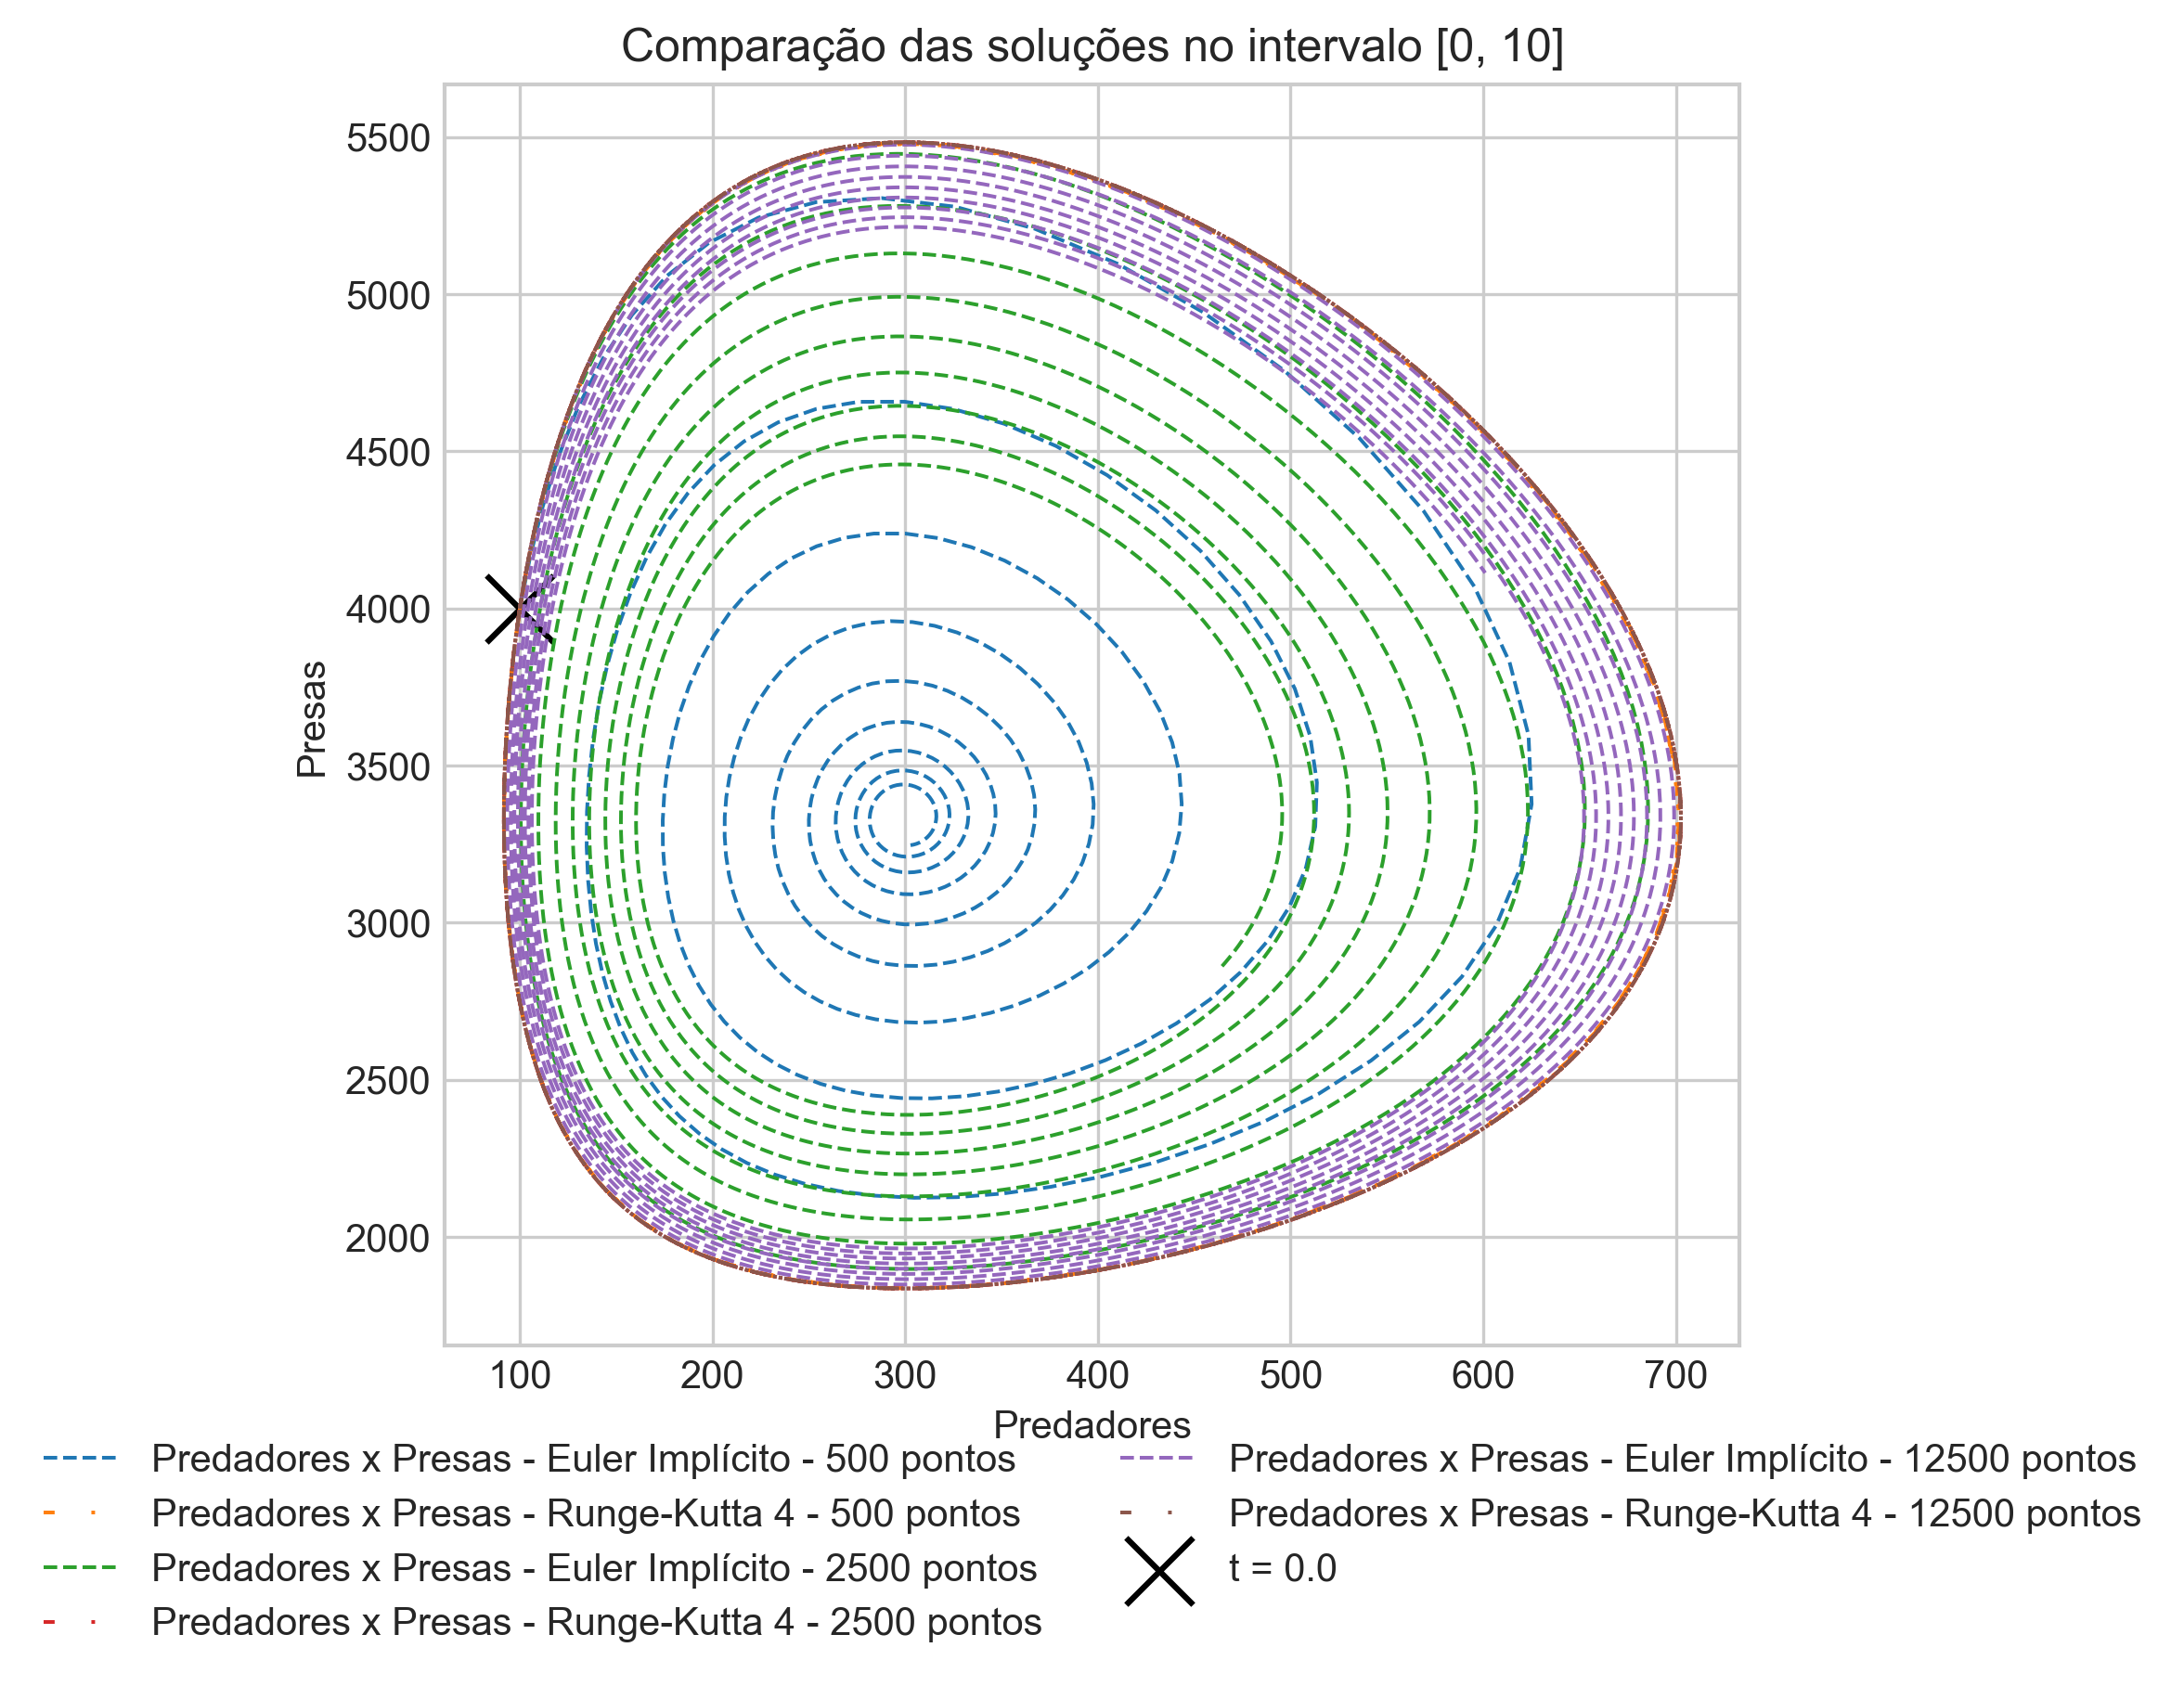
\includegraphics[height=10cm]{predator-prey/pp-comparison-2d.png}}
	}
   \mbox{
		\subfigure[]{
			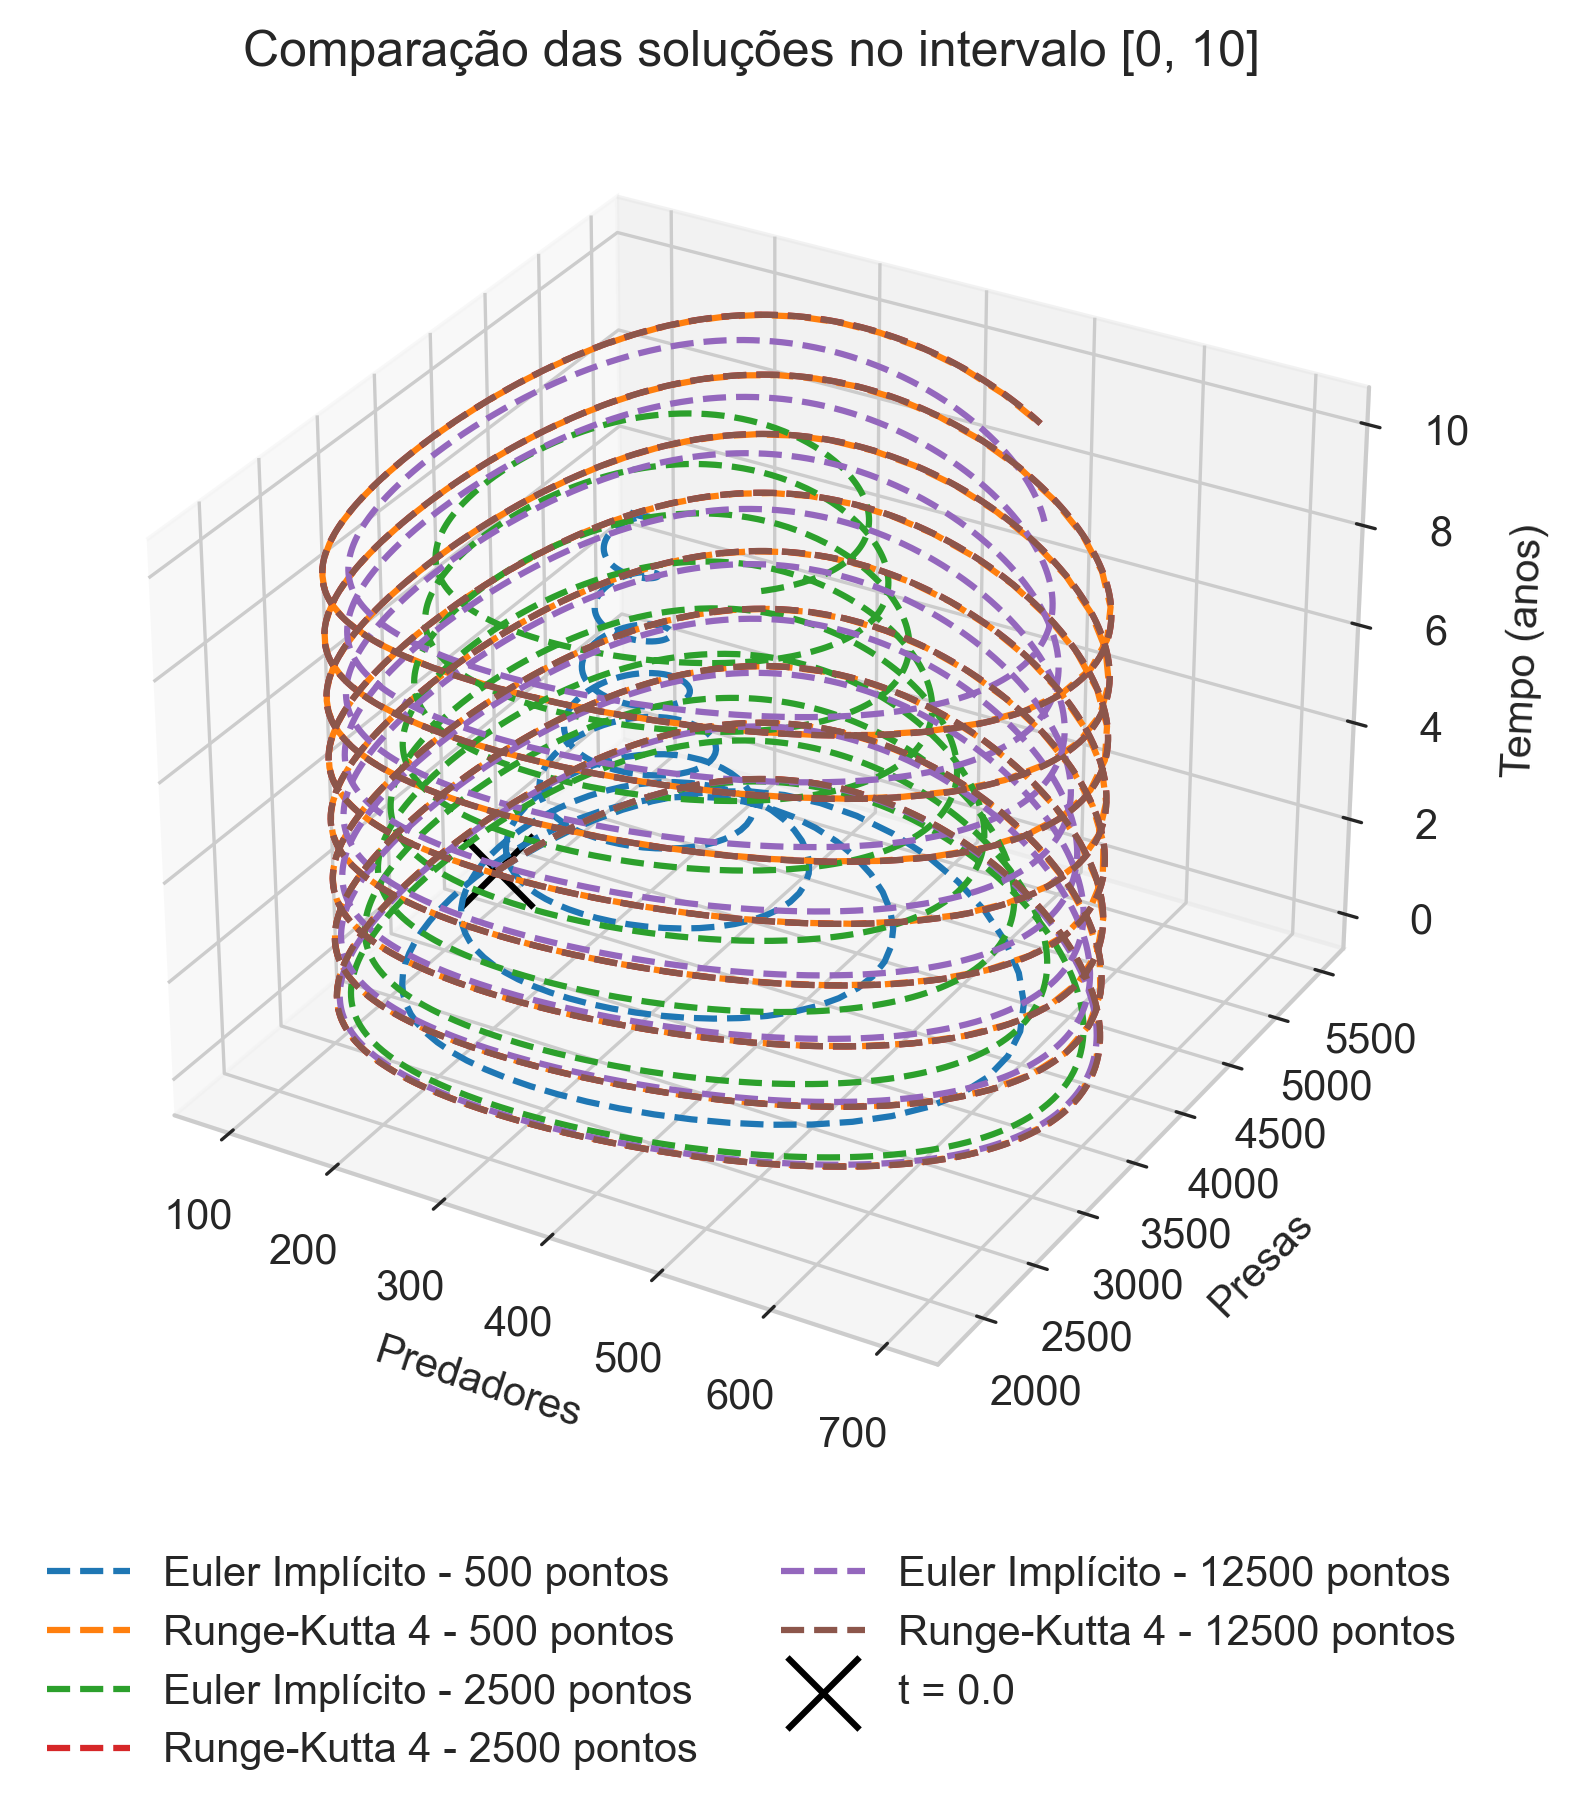
\includegraphics[height=10cm]{predator-prey/pp-comparison.png}}
   }
	\caption{(a) Representação bidimensional das soluções obtidas para distintas malhas; (b) Representação temporal das soluções obtidas}
    \label{img:comparison_plots}
\end{figure}

A Figura \ref{img:comparison_plots} mostra que o método de quarta ordem converge para a mesma solução, independentemente do refinamento da malha, evidenciando sua estabilidade e precisão numérica. Por outro lado, o método implícito apresentou maior sensibilidade ao refinamento da malha, tendo a solução se aproximado daquela obtida pelo método de Runge-Kutta. Apesar disso, o comportamento espiral ainda persiste no método implícito.

\begin{figure}[H]
	\centering
    \mbox{
        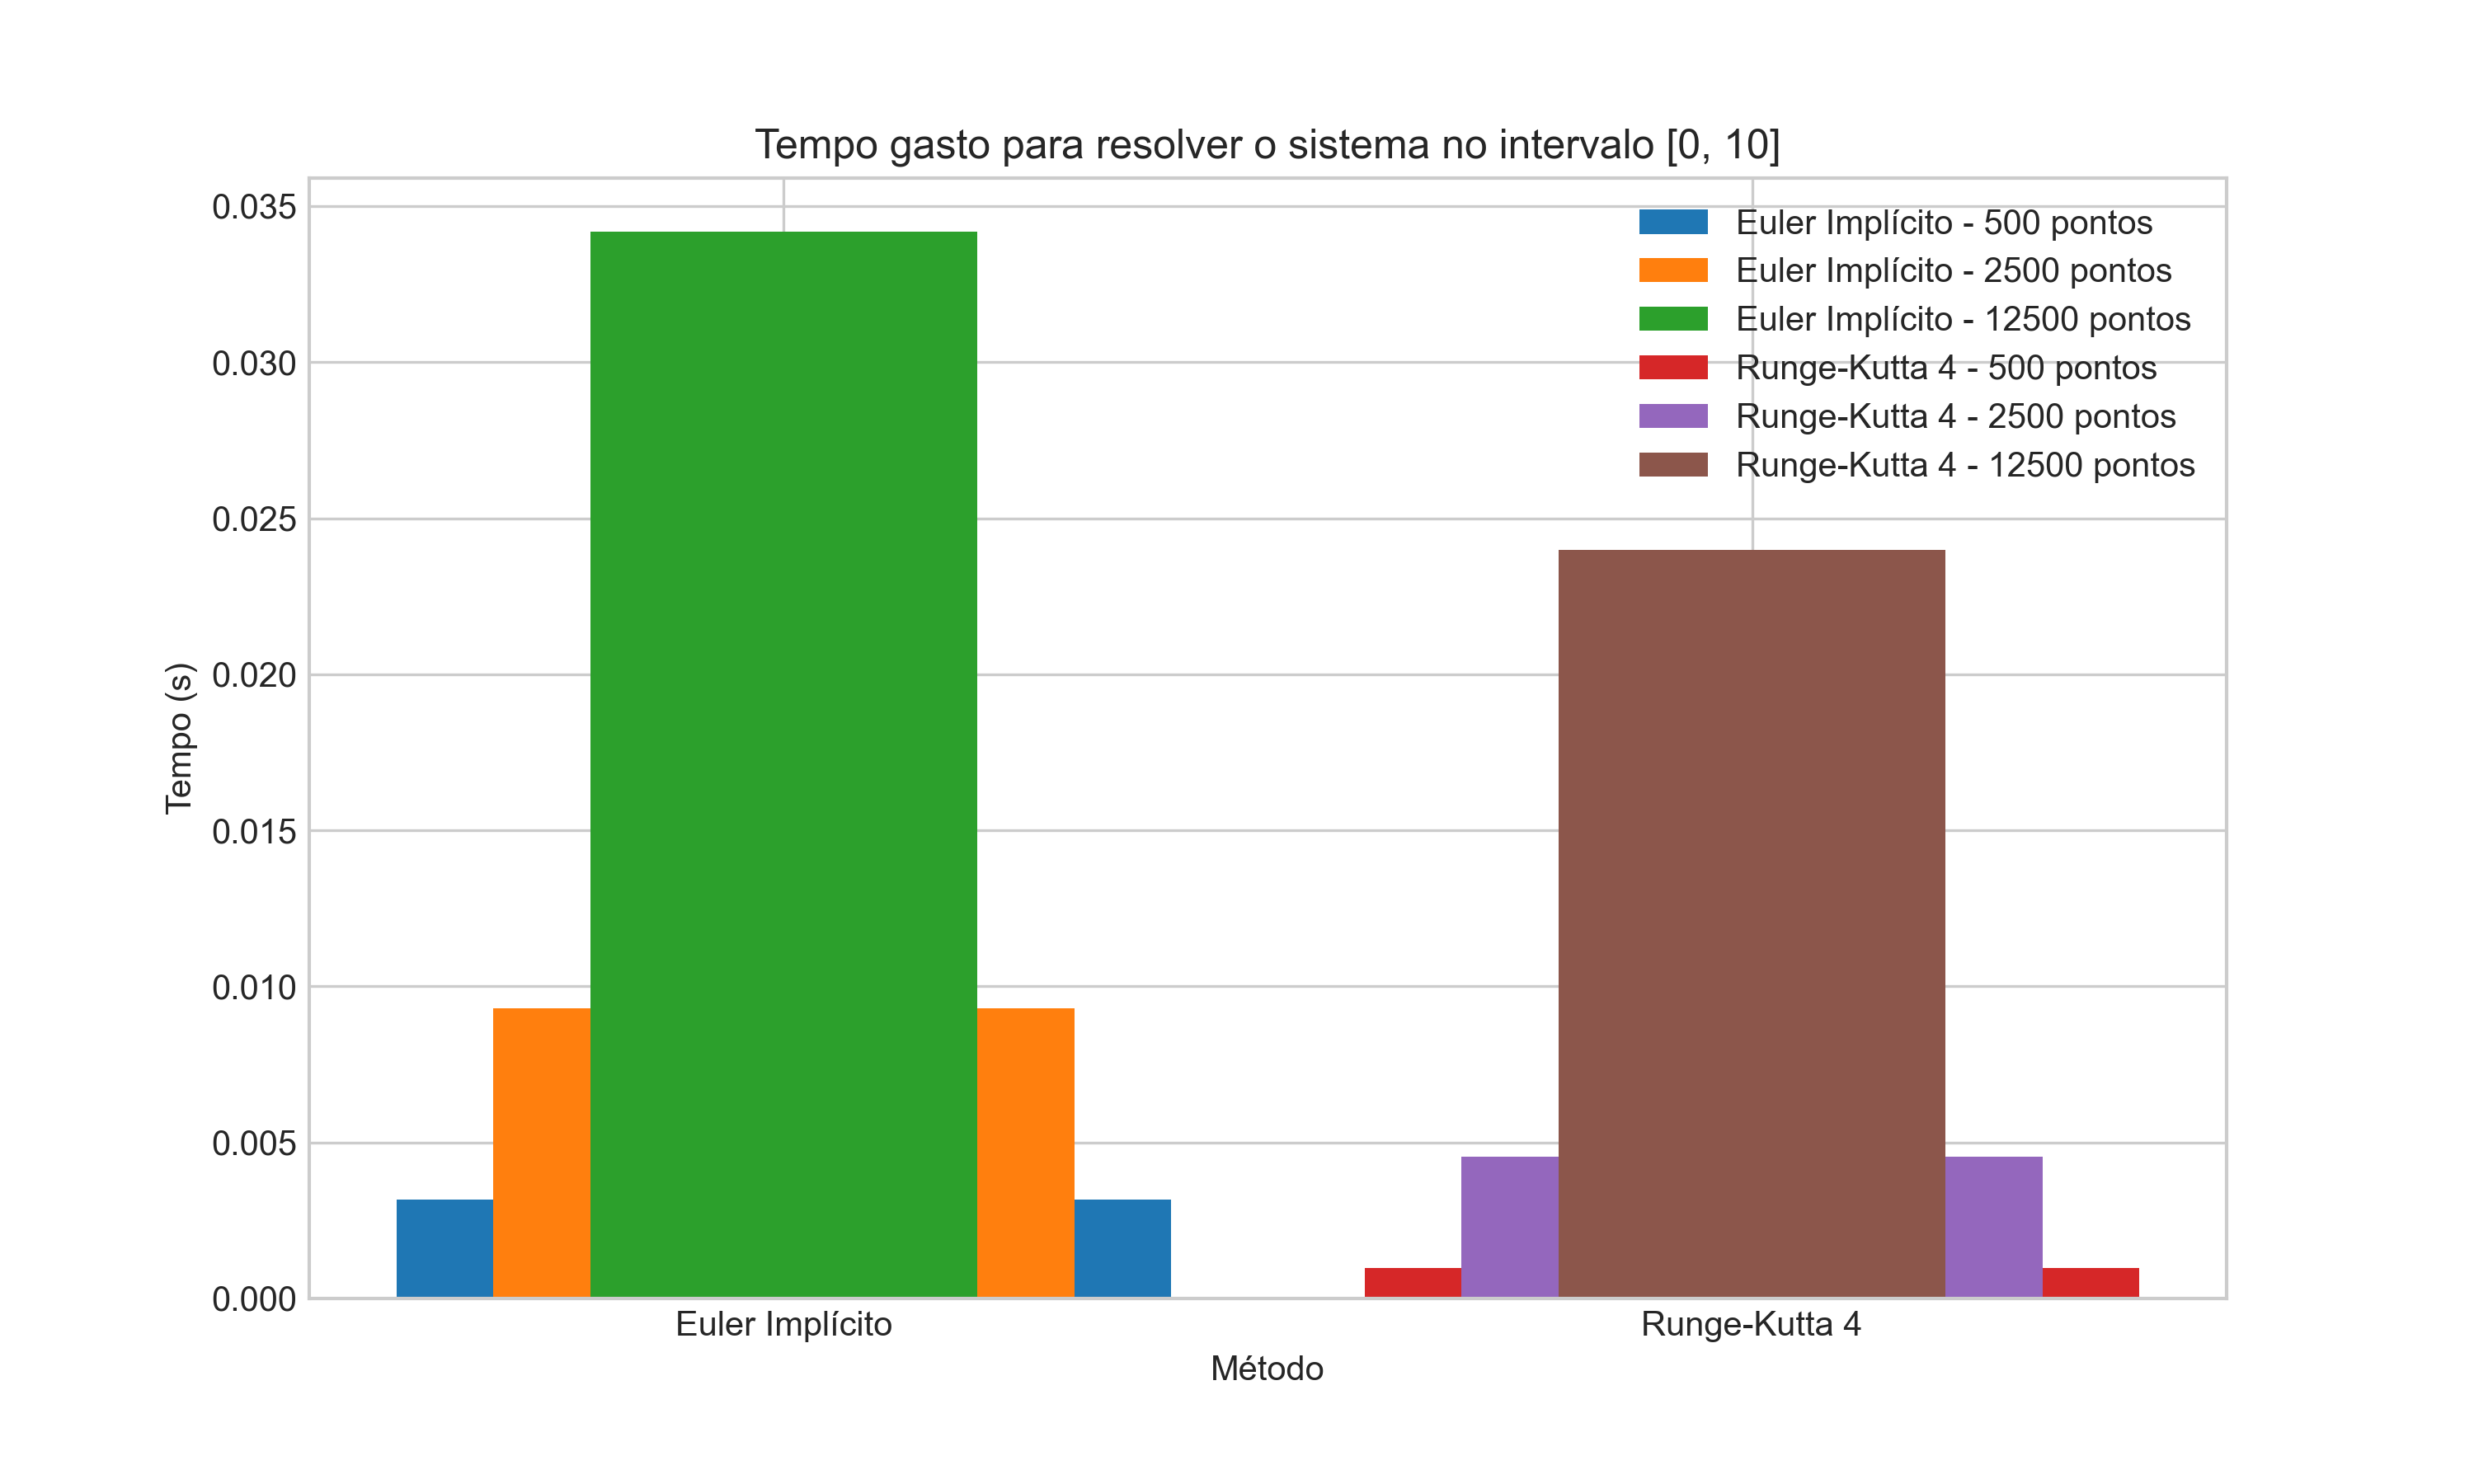
\includegraphics[width=14cm]{predator-prey/predator_prey-300dpi-time-comparison.png}
    }
	\caption{Tempo gasto para resolver o sistema.}
    \label{img:pp-times}
\end{figure}

Considerando a Figura \ref{img:comparison_plots}, é possível observar que ambos os métodos estão convergindo para a solução, porém, em velocidades distintas. É importante destacar que a escolha de um método dependerá da precisão e eficiência computacional desejadas. Nesse sentido, o método de quarta ordem pode ser considerado o mais adequado para este problema, uma vez que obteve uma solução melhor com uma quantidade de pontos bastante inferior ao método de primeira ordem, economizando tempo de processamento computacional, conforme apresentado na Figura \ref{img:pp-times}.
\section{Considerações Finais}\label{sec:conclusion}



Este relatório apresentou a aplicação dos métodos computacionais de diferenças finitas e de Runge-Kutta para a análise temporal do crescimento de uma ou mais populações em um sistema fechado. Esses métodos oferecem uma alternativa vantajosa em relação à solução analítica, que nem sempre é conhecida ou de fácil cálculo.

Para otimizar o desempenho dos algoritmos, foi necessário recorrer à biblioteca de compilação \emph{Just-In-Time} devido à quantidade de tempo necessária para computar os $N$ pontos de cada problema. Além disso, foi utilizada uma escolha particular para resolver a equação implícita do método de Euler Implícito, que aumentou drasticamente o tempo de execução do método. No entanto, se a equação implícita fosse resolvida antes da execução, o tempo gasto em um problema genérico se aproximaria do tempo do método de Euler Explícito. Como evidenciado pelos gráficos apresentados neste trabalho, o método de Euler Implícito é o que consome mais tempo para ser completamente executado.

Em resumo, a aplicação dos métodos computacionais estudados neste trabalho permite o início de uma resolução de problemas complexos do mundo real, oferecendo uma alternativa eficiente e acessível para aproximar numericamente soluções que nem sempre são conhecidas ou de fácil cálculo.

\pagebreak

\bibliography{references}

\end{document}
 
}